%Generazione delle variabili che andranno a sostituire quelle del template 'HomePage.tex'
\newcommand{\documento}{\DDP}
\newcommand{\nomedocumentofisico}{DefinizioneDiProdotto\_v1\_0\_0.pdf}
\newcommand{\redazione}{\FB\\ & \AF\\ & \GN\\ & \GR\\ & \SM\\ & \MP\\ & \MV}
\newcommand{\verifica}{\FB\\ & \AF\\ & \GN}
\newcommand{\approvazione}{\SM}
\newcommand{\uso}{Interno}
\newcommand{\datacreazione}{26 Febbraio 2016}
\newcommand{\datamodifica}{}
\newcommand{\stato}{In redazione}
\newcommand{\destinateTo}{\TV, \\ & \RC, \\ & \ZU}

\def\TABELLE{false}	%abilita - disabilita l'indice delle tabelle
\def\FIGURE{false} 	%abilita - disabilita l'indice delle figure

\documentclass[a4paper,11pt]{article}

%***IMPORTAZIONE PACKAGE***
\usepackage{ifthen}
\usepackage[italian]{babel}
\usepackage[utf8]{inputenc}
\usepackage[T1]{fontenc}
\usepackage{float}
\usepackage{chapterbib}
\usepackage{graphicx}
\usepackage[a4paper,top=2.5cm,bottom=2.5cm,left=2.5cm,right=2.5cm]{geometry}
\usepackage[colorlinks=true, urlcolor=black, citecolor=black, linkcolor=black]{hyperref}
\usepackage{booktabs}
\usepackage{fancyhdr}
\usepackage{totpages}
\usepackage{tabularx, array}
\usepackage{dcolumn}
\usepackage{epstopdf}
\usepackage{booktabs}
\usepackage{fancyhdr}
\usepackage{longtable}
\usepackage{calc}
\usepackage{datatool}
\usepackage[bottom]{footmisc}
\usepackage{listings} 
\usepackage{textcomp}
\usepackage{titlesec}
\usepackage{rotating} 
\usepackage{multirow}
\usepackage{placeins}
\usepackage{color}
\usepackage[table,usenames,dvipsnames]{xcolor}
\usepackage{hyperref}
\usepackage{makecell}
\usepackage{hyperref}


%***STILE PAGINA***
\pagestyle{fancy}
%no indentazione paragrafo
\setlength{\parindent}{0pt}

%***INTESTAZIONE***
\lhead{\Large{\progetto} \\ \footnotesize{\documento}}
\rhead{
\includegraphics[keepaspectratio = true, width = 25px] {../../Template/icone/LogoGruppo.png}}
\renewcommand{\headrulewidth}{0.4pt}  %Linea sotto l'intestazione

%***PIÈ DI PAGINA***
\lfoot{\textit{\gruppoLink}\\ \footnotesize{\email}}
\rfoot{\thepage} %per le prime pagine: mostra solo il numero romano
\cfoot{}
\renewcommand{\footrulewidth}{0.4pt}   %Linea sopra il piè di pagina

%***INSERIMENTO DI NUOVE SOTTOSEZIONI
\setcounter{secnumdepth}{7}		% mostra nel documento fino al livello 8 (1.2.3.4.5.6.7.8)
\setcounter{tocdepth}{7}			% mostra nell'indice fino al livello 8 (1.2.3.4.5.6.7.8)

%***LA SOTTOSEZIONE PARAGRAPH VIENE VISUALIZZATA COME UNA SECTION
\titleformat{\paragraph}{\normalfont\normalsize\bfseries}{\theparagraph}{1em}{}
\titlespacing*{\paragraph}{0pt}{3.25ex plus 1ex minus .2ex}{1.5ex plus .2ex}

\titleformat{\subparagraph}{\normalfont\normalsize\bfseries}{\thesubparagraph}{1em}{}
\titlespacing*{\subparagraph}{0pt}{3.25ex plus 1ex minus .2ex}{1.5ex plus .2ex}

\makeatletter
\newcounter{subsubparagraph}[subparagraph]
\renewcommand\thesubsubparagraph{%
  \thesubparagraph.\@arabic\c@subsubparagraph}
\newcommand\subsubparagraph{%
  \@startsection{subsubparagraph}    % counter
    {6}                              % level
    {\parindent}                     % indent
    {3.25ex \@plus 1ex \@minus .2ex} % beforeskip
    {0.75em}                           % afterskip
    {\normalfont\normalsize\bfseries}}
\newcommand\l@subsubparagraph{\@dottedtocline{6}{10em}{5.5em}} %gestione dell'indice
\newcommand{\subsubparagraphmark}[1]{}
\makeatother

\makeatletter
\newcounter{subsubsubparagraph}[subsubparagraph]
\renewcommand\thesubsubsubparagraph{%
  \thesubsubparagraph.\@arabic\c@subsubsubparagraph}
\newcommand\subsubsubparagraph{%
  \@startsection{subsubsubparagraph}    % counter
    {7}                              % level
    {\parindent}                     % indent
    {3.25ex \@plus 1ex \@minus .2ex} % beforeskip
    {0.75em}                           % afterskip
    {\normalfont\normalsize\bfseries}}
\newcommand\l@subsubsubparagraph{\@dottedtocline{7}{10em}{6.5em}} %gestione dell'indice
\newcommand{\subsubsubparagraphmark}[1]{}
\makeatother
%Generali
\newcommand{\progetto}{QuizziPedia}
\newcommand{\gruppo}{TheFellowshipOfTheCode}
\newcommand{\gruppoLink}{\href{http://thefellowshipofthecode.github.io/}{TheFellowshipOfTheCode}}
\newcommand{\email}{\href{mailto:thefellowshipofthecode@gmail.com}{thefellowshipofthecode@gmail.com}}

%Documenti
\newcommand{\AdR}{Analisi dei Requisiti}
\newcommand{\NdP}{Norme di Progetto}
\newcommand{\PdP}{Piano di Progetto}
\newcommand{\SdF}{Studio di Fattibilità}
\newcommand{\PdQ}{Piano di Qualifica}
\newcommand{\VI}{Verbale Interno}
\newcommand{\VE}{Verbale Esterno}
\newcommand{\ST}{Specifica Tecnica}
\newcommand{\DDP}{Definizione di Prodotto}
\newcommand{\MU}{Manuale Utente}
\newcommand{\G}{Glossario}
\newcommand{\LdP}{Lettera di Presentazione}
\newcommand{\NdPv}{NormeDiProgetto\_v\_1\_0\_0}
\newcommand{\PdPv}{PianoDiProgetto\_v\_1\_0\_0}
\newcommand{\PdQv}{PianoDiQualifica\_v\_1\_0\_0}
\newcommand{\SdFv}{StudioDiFattibilità\_v\_1\_0\_0}

%Componenti del gruppo
\newcommand{\AF}{Alberto Ferrara}
\newcommand{\SM}{Simone Magagna}
\newcommand{\FB}{Franco Berton}
\newcommand{\MP}{Marco Prelaz}
\newcommand{\MV}{Mattia Varotto}
\newcommand{\GN}{Matteo Gnoato}
\newcommand{\GR}{Matteo Granzotto}

%Ruoli
\newcommand{\RdP}{Responsabile di Progetto}
\newcommand{\Res}{Responsabile}
\newcommand{\Amm}{Amministratore}
\newcommand{\Ver}{Verificatore}
\newcommand{\Prog}{Progettista}
\newcommand{\Progr}{Programmatore}
\newcommand{\Ana}{Analista}
\newcommand{\RdPs}{Responsabili di Progetto}
\newcommand{\Ress}{Responsabile}
\newcommand{\Amms}{Amministratori}
\newcommand{\Vers}{Verificatori}
\newcommand{\Progs}{Progettisti}
\newcommand{\Progrs}{Programmatori}
\newcommand{\Anas}{Analisti}

%Professori e proponente
\newcommand{\TV}{Prof. Tullio Vardanega}
\newcommand{\RC}{Prof. Riccardo Cardin}
\newcommand{\ZU}{Zucchetti S.P.A.}
\newcommand{\proponente}{Zucchetti S.P.A.}

\newcommand{\diaryEntry}[5]{#2 & \emph{#4} & #3 & #5 & #1\\ \hline}

%comando per una nuova riga nella tabella del diario delle modifiche
\newcommand{\specialcell}[2][c]{%
	\begin{tabular}[#1]{@{}c@{}}#2\end{tabular}}

\renewcommand*\sectionmark[1]{\markboth{#1}{}}
\renewcommand*\subsectionmark[1]{\markright{#1}}

%Pediodi di lavoro 
\newcommand{\AR}{Analisi dei Requisiti}
\newcommand{\AD}{Analisi dei Requisiti in Dettaglio}
\newcommand{\PA}{Progettazione Architetturale}
\newcommand{\PD}{Progettazione di Dettaglio}
\newcommand{\CO}{Codifica}
\newcommand{\VV}{Verifica e Validazione}

% Revisioni
\newcommand{\RR}{Revisione dei Requisiti}
\newcommand{\RP}{Revisione di Progettazione}
\newcommand{\RQ}{Revisione di Qualifica}
\newcommand{\RA}{Revisione di Accettazione}

% Comandi analisi dei requisiti
\newcommand{\uau}{utente autenticato}
\newcommand{\uaus}{utenti autenticati}
\newcommand{\uaupro}{utente autenticato pro}
\newcommand{\uauspro}{utenti autenticati pro}

\newcommand{\myincludegraphics}[2][]{%
	\setbox0=\hbox{\phantom{X}}%
	\vtop{
		\hbox{\phantom{X}}
		\vskip-\ht0
		\hbox{\includegraphics[#1]{#2}}}}

\newcommand{\modificheuno} 
{	
	0.0.3 & Inseriti i primi riferimenti informativi & \specialcell[t]{\GN \\ \prog} & 2016-02-26
	\\\midrule
	0.0.2 & Stesura scopo del documento, scopo del prodotto , riferimenti normativi & \specialcell[t]{\GN \\ \prog} & 2016-02-26
	\\\midrule
	0.0.1 & Creato template documento & \specialcell[t]{\GN \\ \prog} & 2016-02-26
	\\\midrule
}
\newcommand{\modifichedue}
{
}
\setcounter{secnumdepth}{7}
\setcounter{tocdepth}{7}
\begin{document}

%inclusione template HomePage
\begin{center}

%
\includegraphics[width=1em]{../../../Template/icone/LogoGruppo.png}
\begin{large} \textbf{\gruppoLink} \end{large}
%
\includegraphics[width=1em]{../../../Template/icone/LogoGruppo.png}
\vspace{0.2em}

\hrule
\vspace{3em}


\includegraphics[keepaspectratio = true, width=8cm]{../../../Template/icone/LogoGruppo.png}

%Prima pagina senza intestazione né piè di pagina	
\thispagestyle{empty}

%Le informazioni del documento sono ancorate a fine pagina
\vfill

%Copertina
\begin{center} 
  \begin{Huge}
  {\fontsize{15mm}{20mm}\selectfont \progetto} 
  \end{Huge}
\end{center}

\begin{Huge} \documento \end{Huge}

\begin{center}
\textbf{Informazioni sul documento} \\ \vspace{2em}
\small
\begin{tabular}{r|l}
	\textbf{Nome Documento} & \nomedocumentofisico \\
	\textbf{Versione}	& 1\\
	\textbf{Data di Creazione} & \datacreazione\\
	\textbf{Data ultima modifica} & \datamodifica\\
	\textbf{Stato} & \stato \\
	\textbf{Redazione}	& \redazione\\
	\textbf{Verifica}	& \verifica\\
	\textbf{Approvazione}	& \approvazione\\
	\textbf{Uso}  & \uso\\
	\textbf{Distribuzione} & \gruppo \\
	\textbf{Destinato a}  &  \destinateTo \\
	\textbf{Email di riferimento} & \email
\end{tabular}
\end{center}

\normalsize
%Sommario
\textbf{Sommario\\} 
Documento contenente le norme di progetto che il gruppo \textit{\gruppo} seguirà durante tutte le fasi di realizzazione del prodotto \textit{\progetto}.

%\vfill %cosa fa?
\end{center}
\clearpage


%Registro delle modifiche e indice 
%si usa la numerazione romana per gli indici e la tabella delle modifiche
\pagenumbering{Roman}
%\newpage
%***REGISTRO DELLE MODIFICHE***
%Vari comandi per la struttura della tabella, NON MODIFICARE!
\begin{center}
	\Large{\textbf{Registro delle modifiche}}
	\\\vspace{0.5cm}
	\normalsize
	\begin{tabularx}{\textwidth}{cXcc}
		\textbf{Versione} & \textbf{Descrizione} & \textbf{Autore e Ruolo} & \textbf{Data} \\\toprule
		\modifiche
		\bottomrule
\end{tabularx}
\end{center}
\newpage
\newpage
%***REGISTRO DELLE MODIFICHE***
%Vari comandi per la struttura della tabella, NON MODIFICARE!
\begin{center}
	\Large{\textbf{Registro delle modifiche}}
	\\\vspace{0.5cm}
	\normalsize
	\begin{tabularx}{\textwidth}{cXcc}
		\textbf{Versione} & \textbf{Descrizione} & \textbf{Autore e Ruolo} & \textbf{Data} \\\toprule
		\modificheuno
		\bottomrule
	\end{tabularx}
	\newpage
	\begin{tabularx}{\textwidth}{cXcc}
		\textbf{Versione} & \textbf{Descrizione} & \textbf{Autore e Ruolo} & \textbf{Data} \\\toprule
		\modifichedue
		\bottomrule
	\end{tabularx}	
\end{center}
\newpage
%Inserisce il link all'indice
%\addcontentsline{toc}{section}{Indice}
\tableofcontents
\clearpage 

%Se è stata impostata a true la variabile per la lista delle tabelle, la mostra
\ifthenelse{\equal{\TABELLE}{true}} 
{\listoftables \newpage}{}

%Se è stata impostata a true la variabile per la lista delle figure, la mostra
\ifthenelse{\equal{\FIGURE}{true}}
{\listoffigures \newpage}{}

%Da qui comincia la numerazione normale
\pagenumbering{arabic}

%Imposta il formato di visualizzazione
\rfoot{\thepage~di~\pageref{TotPages}}

\newpage 
\listoffigures
\newpage
\listoftables
\newpage

\newpage
\section{Introduzione}

\subsection{Scopo del documento}
Il presente documento ha lo scopo di definire in dettaglio la struttura e il funzionamento delle componenti del progetto \progetto. Questo documento servirà come guida per i \textit{\Progrs} del gruppo \gruppo fornendo direttive e vincoli per la realizzazione del \textit{progetto\ped{G}}.

\subsection{Scopo del prodotto}
Lo scopo del prodotto è di permettere la creazione e gestione di questionari in grado di identificare le lacune dei candidati prima, durante e al termine di un corso di formazione. 
\\Il sistema dovrà offrire le seguenti funzionalità:
\begin{itemize}
	\item
	Archiviare questionari in un server suddivisi per argomento;
	\item
	Somministrare all'utente, tramite un'interfaccia, questionari specifici per argomento scelto;
	\item
	Verificare e valutare i questionari scelti dagli utenti in base alle risposte date.
\end{itemize}
La parte destinata ai creatori di questionari dovrà essere fruibile attraverso un \textit{browser\ped{G}} desktop, abilitato all'utilizzo delle tecnologie \textit{HTML5\ped{G}}, \textit{CSS3\ped{G}} e \textit{JavaScript\ped{G}}. La parte destinata agli esaminandi sarà utilizzabile su qualunque dispositivo: dal personal computer ai tablet e smartphone.

\subsection{Glossario}
Al fine di evitare ogni ambiguità i termini tecnici del dominio del progetto, gli acronimi e le parole che necessitano di ulteriori spiegazioni saranno nei vari documenti marcate con il pedice \ped{G} e quindi presenti nel documento \textit{\G}.


\subsection{Riferimenti}
\subsubsection{Normativi}
\begin{itemize}
	\item \textit{\NdPv};
	\item \textit{\AdRvDue};
\end{itemize}
\subsubsection{Informativi}
\begin{itemize}
	\item \textbf{Ingegneria del software - Ian Sommerville - 8a edizione (2007)}: \\
	Parte terza: Progettazione, capitolo 11: Progettazione architetturale, Capitolo 14: Progettazione orientata agli oggetti;
	\item \textbf{Design Patterns} - Erich Gamma, Richard Helm, Ralph Johnson, John Vlissides - 1a edizione italiana (2006);
	\item \textbf{Slide dell'insegnamento - Design patterns:}
	\begin{itemize}
		\item Strutturali: \url{http://www.math.unipd.it/~tullio/IS-1/2015/Dispense/E07.pdf};
		\item Creazionali: \url{http://www.math.unipd.it/~tullio/IS-1/2015/Dispense/E08.pdf}
		\item Comportamentali: \url{http://www.math.unipd.it/~tullio/IS-1/2015/Dispense/E09.pdf}
		\item Architetturali:
			\begin{itemize}
				\item \url{http://www.math.unipd.it/~rcardin/sweb/Design%20Pattern%20Architetturali%20-%20Model%20View%20Controller_4x4.pdf};
				\item \url{http://www.math.unipd.it/~rcardin/sweb/Design%20Pattern%20Architetturali%20-%20Dependency%20Injection_4x4.pdf}.
			\end{itemize} 
	\end{itemize}
	\item \textbf{Martin Fowler - UML\ped{G} Distilled} - 2nd edition;
	\item \textbf{Slide dell'insegnamento - Diagrammi delle classi}: \\
		\url{http://www.math.unipd.it/~tullio/IS-1/2015/Dispense/E03.pdf}
	\item \textbf{Slide dell'insegnamento - Diagrammi dei packages:} \\
		\url{http://www.math.unipd.it/~tullio/IS-1/2015/Dispense/E04.pdf}
	\item \textbf{Slide dell'insegnamento - Diagrammi di sequenza:} \\
		\url{http://www.math.unipd.it/~tullio/IS-1/2015/Dispense/E05.pdf}
	\item \textbf{Documentazione del \textit{Framework\ped{G}MEAN\ped{G}.js}:} \\
		\url{http://learn.mean.io/}
	\item \textbf{Documentazione della \textit{piattaforma} Node.js:} \\
		\url{https://nodejs.org/api/}
	\item \textbf{Giuda all'utilizzo dei middleware Express:} \\
		\url{http://expressjs.com/it/guide/using-middleware.html}
	\item \textbf{Guida all'utilizzo dei middleware Passport:} \\
		\url{http://passportjs.org/docs}
	\item \textbf{Manuale del database \textit{MongoDB\ped{G}}:} \\
		\url{https://docs.mongodb.org/manual/}
	\item \textbf{Documentazione dell'interfaccia REST:}
		\begin{itemize}
			\item \textit{Descrizione di REST:} \url{https://it.wikipedia.org/wiki/Representational_State_Transfer}
			\item \textit{Descrizione risorse REST:} \url{http://stashboard.readthedocs.org/en/latest/restapi.html}
		\end{itemize}
	\item \textbf{Documentazione del \textit{framework\ped{G} AngularJS\ped{G}}:} \\
		\begin{itemize}
			\item \textit{Documentazione generica:} \url{https://docs.angularjs.org/guide}
			\item \textit{Documentazione servizio \$http:} \url{https://docs.angularjs.org/api/ng/service/\$http}
			\item \textit{Documentazione servizio \$location:} \url{https://docs.angularjs.org/api/ng/service/\$location}
			\item \textit{Documentazione servizio \$windows:} \url{https://docs.angularjs.org/api/ng/service/\$window}
			\item \textit{Documentazione servizio \$ruoteParams:} \url{https://docs.angularjs.org/api/ngRoute/service/\$routeParams}
			\item \textit{Documentazione servizio \$q:} \url{https://docs.angularjs.org/api/ng/service/\$q}
		\end{itemize}
	\item \textbf{Documentazione del \textit{framework\ped{G}} Material for Angular:} \\
		\url{https://material.angularjs.org/latest/}
	\item \textbf{Documentazione del \textit{framework\ped{G}} Chart.js} \\
		\url{http://www.chartjs.org/docs/}
	\item \textbf{Documentazione del \textit{wrapper\ped{G}} Angles.js} \\
		\url{https://github.com/gonewandering/angles}
	\item \textbf{Documentazione del \textit{framework\ped{G}} TextAngular.js} \\
		\url{https://github.com/fraywing/textAngular/wiki/textAngular-Docs-v1.1.x}
	\item \textbf{Guida all'utilizzo della direttiva \textit{ng-file-upload}} \\
		\url{https://github.com/danialfarid/ng-file-upload}
	\item \textbf{Documentazione di \textit{jison\ped{G}} per la definizione della grammatica di QML} \\
		\url{http://zaa.ch/jison/docs/}
\end{itemize}
\newpage
\section{Descrizione generale}
\subsection{Contesto d'uso del prodotto}
\subsection{Funzioni del prodotto}
\subsection{Caratteristiche degli utenti}
\subsection{Vincoli generali}
\subsection{Assunzione dipendenze}

\newpage
\section{QuizziPedia::Front-End}
\label{QuizziPedia::Front-End}
\begin{figure}[ht]
	\centering
	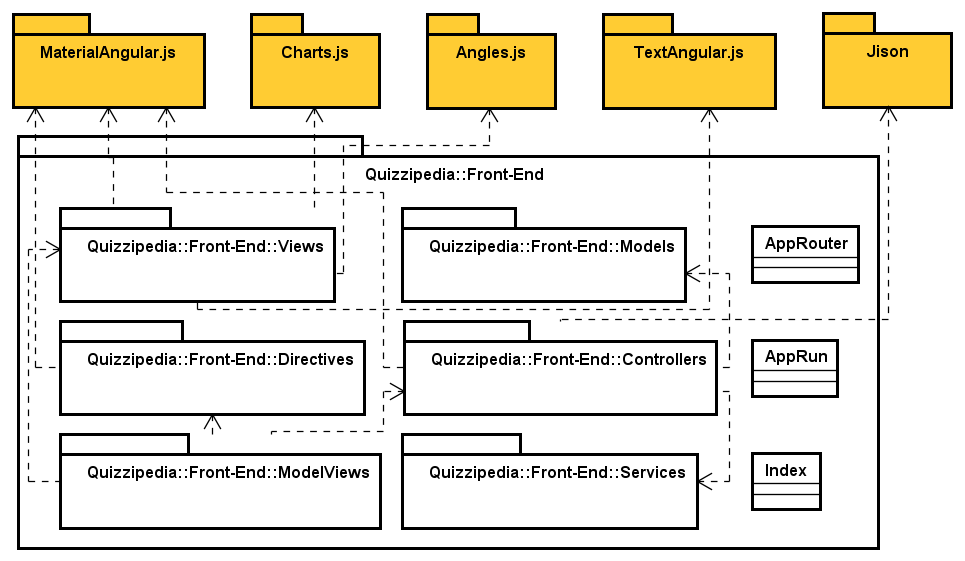
\includegraphics[scale=0.35]{UML/Package/QuizziPedia_Front-end.png}
	\caption{QuizziPedia::Front-End}
\end{figure}
\FloatBarrier
\begin{itemize}
	\item \textbf{Descrizione}: \textit{package\ped{G}} contenente le componenti front-end dell'applicazione;
	\item \textbf{Package contenuti}:
	\begin{itemize}
		\item \texttt{Views}: \textit{package\ped{G}} contenente le \textit{views\ped{G}} front-end dell'applicazione;
		\item \texttt{Controllers}: \textit{package\ped{G}} contenente i \textit{controllers\ped{G}} front-end dell'applicazione;
		\item \texttt{Services}: \textit{package\ped{G}} contenente i \textit{services\ped{G}} front-end dell'applicazione;
		\item \texttt{Models}: \textit{package\ped{G}} contenente le classi che definiscono la business logic dell'applicazione;
		\item \texttt{Directives}: \textit{package\ped{G}} contenente le \textit{directives\ped{G}} front-end dell'applicazione.
	\end{itemize}
	\item \textbf{Classi contenute}:
	\begin{itemize}
		\item \texttt{Index}: \textit{view\ped{G}} generale dell'applicazione. Contiene gli elementi che saranno presenti in ogni pagina dell'applicazione;
		\item \texttt{AppRun}: classe che verifica se l'utente sia autenticato e che abbia le giuste autorizzazioni per la pagina in cui si trova;
		\item \texttt{AppRouter}: classe che gestisce i routes dell'applicazione, utilizza il servizio \$routeProvider per associare ad ogni route un \textit{controller\ped{G}} e una \textit{view\ped{G}}.
	\end{itemize}
\end{itemize}

\newpage
\subsection{QuizziPedia::Front-End::Views}

\label{QuizziPedia::Front-End::Views}
\begin{figure}[ht]
	\centering
	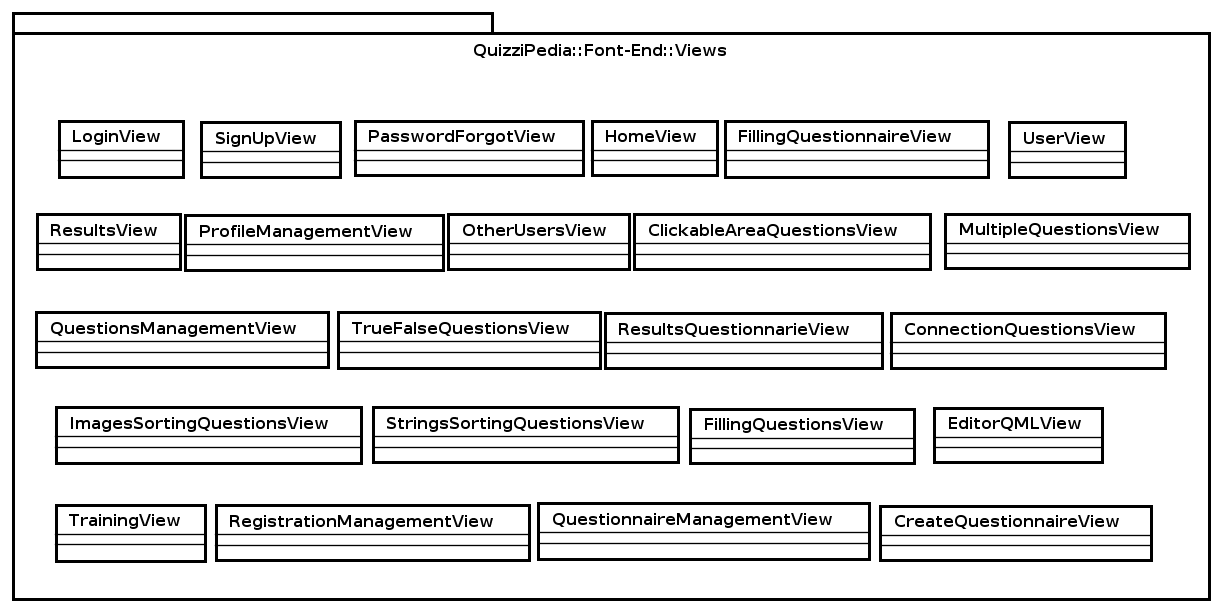
\includegraphics[scale=0.55]{UML/Package/QuizziPedia_Front-End_Views.png}
	\caption{QuizziPedia::Front-End::Views}
\end{figure}\FloatBarrier
\begin{itemize}
	\item \textbf{Descrizione}: package contenente le views front-end dell'applicazione;
	\item \textbf{Padre}: \texttt{Front-End};
	\item \textbf{Interazione con altri componenti}:
	\begin{itemize}
		\item \texttt{Controllers}: package contenente i \textit{controllers\ped{G}} Front-End dell'applicazione;
		\item \texttt{Directives}: package contenente le \textit{directives\ped{G}} Front-End dell'applicazione.
	\end{itemize}
	\item \textbf{Classi contenute}:
	\begin{itemize}
		\item \texttt{LoginView}: classe contenente le form necessarie per effettuare il login. Contiene inoltre un link alla pagina di registrazione e uno alla pagina per il recupero della password;
		\item \texttt{SignUpView}: classe contenente le form dedicate alla registrazione utente. Contiene inoltre un link alla pagina di login;
		\item \texttt{PasswordForgotView}: classe contenente le form necessarie per il recupero della password dimenticata;
		\item \texttt{HomeView}: classe contenente la direttiva per barra di ricerca degli utenti e questionari e il bottone che porterà l'utente nella modalità allenamento;
		\item \texttt{ResultsView}: classe contenente i risultati della ricerca effettuata. Vengono visualizzati sia gli utenti che i questionari trovati;
		\item \texttt{UserView}: contenente le direttive dei dati personali dell'utente, delle sue statistiche relative ai questionari e agli allenamenti effettuati e dei questionari a cui è iscritto;
		\item \texttt{OtherUserView}: classe contenente le direttive dei dati personali e delle statistiche di un utente ricercato;
		\item \texttt{ProfileManagementView}: classe contenente i dati personali che un utente può modificare dopo essersi registrato al sistema;
		\item \texttt{QuestionsManagementView}: classe contenente l'elenco delle domande create;
		\item \texttt{TrueFalseQuestionView}: classe contenente le direttive per creare una domanda vero/falso;
		\item \texttt{MultipleQuestionView}: classe contenente le direttive per creare una domanda a risposta multipla;
		\item \texttt{ConnectionQuestionView}: classe contenente i campi e le direttive per creare una domanda a collegamento;
		\item \texttt{ImagesSortingQuestionView}: classe contenente i campi e le direttive per creare una domanda a ordinamento immagini;
		\item \texttt{StringsSortingQuestionView}: classe contenente i campi e le direttive per creare una domanda a ordinamento stringhe;
		\item \texttt{FillingQuestionsView}: classe contenente i campi e le direttive per creare una domanda a riempimento testo;
		\item \texttt{ClickableAreaQustionView}: classe contenente i campi e le direttive per creare una domanda ad area cliccabile;
		\item \texttt{EditorQMLView}: classe contenente l'editor \textit{QML\ped{G}} per la creazione di domande personalizzate;
		\item \texttt{TrainingView}: classe principale della modalità allenamento; conterrà i vari templates di ogni domanda dell'allenamento;
		\item \texttt{FillingQuestionnaireView}: classe principale per la compilazione del questionario; conterrà i vari templates di ogni domanda appartenente al questionario;
		\item \texttt{QuestionnaireManagementView}: classe principale per la gestione dei questionari;
		\item \texttt{CreateQuestionnaireView}: classe per la creazione del questionario;
		\item \texttt{ResultQuestionnaireView}: classe contenente i risultati conseguiti dagli utenti che hanno compilato il proprio questionario;
		\item \texttt{RegiastrationManagementView}: classe che permette di visualizzare gli utenti iscritti ad un questionario.
	\end{itemize}
\end{itemize}
\newpage
\subsection{QuizziPedia::Front-End::Controllers}

\begin{figure} [ht]
	\centering
	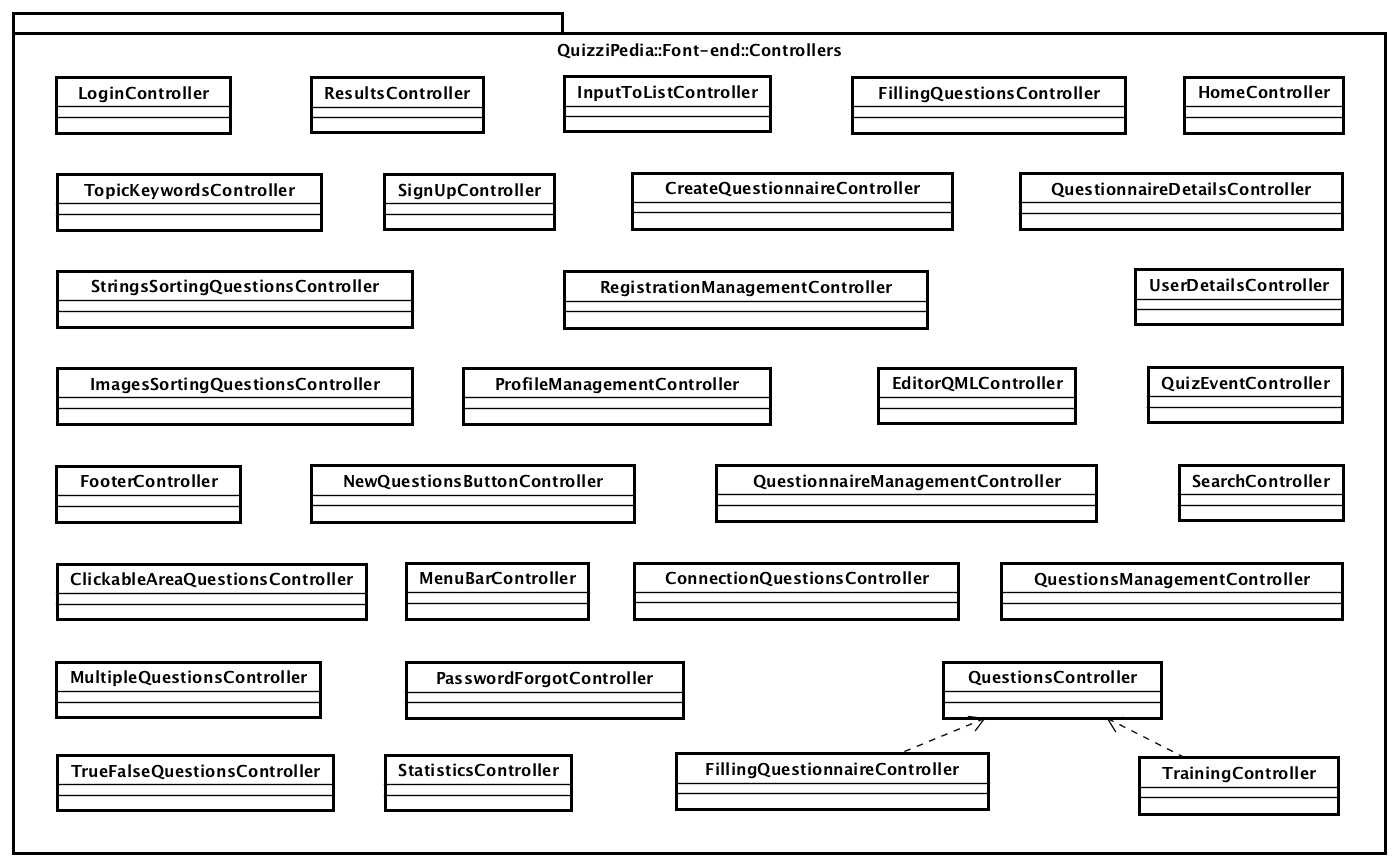
\includegraphics[scale=0.45]{UML/Package/QuizziPedia_Front-End_Controllers.png}
	\caption{QuizziPedia::Front-End::Controllers}
\end{figure} \FloatBarrier

\begin{itemize}
	\item \textbf{Descrizione}: \textit{package\ped{G}} che contiene i controller individuati per la parte front-end dell'applicazione;
	\item \textbf{Padre}: \texttt{Front-End};
	\item \textbf{Interazione con altri componenti}:
	\begin{itemize}
		\item \texttt{Views}: \textit{package\ped{G}} che contiene le \textit{views\ped{G}} dell'applicazione;
		\item \texttt{Models}: \textit{package\ped{G}} che contiene le classi \textit{model\ped{G}} dell'applicazione;
		\item \texttt{Services}: \textit{package\ped{G}} che contiene i \textit{services\ped{G}} dell'applicazione.
	\end{itemize}
	\item \textbf{Classi contenute}:
	\begin{itemize}
		\item \texttt{ClickableAreaQuestionController}: questa classe permette di gestire la creazione e la modifica di una domanda ad area cliccabile;
		\item \texttt{ConnectionQuestionController}: questa classe permette di gestire la creazione e la modifica di una domanda a collegamento;
		\item \texttt{CreateQuesrtionnaireController}: questa classe permette di gestire la creazione di un questionario;
		\item \texttt{EditorQMLController}: questa classe permette di gestire la creazione e la modifica di domande create tramite editor \textit{QML\ped{G}};
		\item \texttt{FillingQuestionnaireController}: questa classe permette di gestire la compilazione del questionario;
		\item \texttt{FillingQuestionsController}: questa classe permette di gestire la creazione e la modifica di una domanda	a riempimento di spazi;
		\item \texttt{HomeController}: questa classe permette di gestire la home page;
		\item \texttt{ImagesSortingQuestionsController}: questa classe permette di gestire la creazione e la modifica di una domanda a ordinamento immagini;
		\item \texttt{InputToListController}: questa classe permette di gestire l'inserimento di una lista di risposte durante la creazione di una domanda;
		\item \texttt{LoginController}: questa classe permette di gestire l'autenticazione dell'utente al sistema;
		\item \texttt{MenuBarController}: questa classe permette di gestire il menù fisso per ogni pagina;
		\item \texttt{MultipleQuestionController}: questa classe permette di gestire la creazione e la modifica di una domanda a risposta multipla;
		\item \texttt{NewQuestionButtonController}: questa classe permette di effettuare il redirect alla pagina di creazione nuova domanda;
		\item \texttt{PasswordForgotController}: questa classe permette di gestire il ripristino della password dimenticata;
		\item \texttt{ProfileManagementController}: questa classe permette di gestire il profilo personale di un utente;
		\item \texttt{QuestionnaireDeatailsController}: questa classe permette di gestire i dettagli di un questionario;
		\item \texttt{QuestionnaireManagementController}: questa classe permette di gestire tutti i questionari creati da un utente;
		\item \texttt{QuestionsController}: questa classe permette di gestire il recupero delle domande per far si che possano essere visualizzate nella modalità allenamento e nella compilazione dei questionari;
		\item \texttt{QuestionsManagementController}: questa classe permette di gestire le domande create dall'utente e di crearne di nuove;
		\item \texttt{QuizEventController}: questa classe permette di reagire ai comandi dell'utente durante la gestione dei suoi questionari;
		\item \texttt{RegistrationManagementController}: questa classe permette di gestire le iscrizione degli utenti ai questionari;
		\item \texttt{ResultQuestionnaireController}: questa classe permette di gestire la visualizzazione dei risultati di un singolo questionario;
		\item \texttt{SearchController}: questa classe permette di gestire la ricerca di questionari e utenti all'interno dell'applicazione;
		\item \texttt{SignUpController}: questa classe permette di gestire la registrazione di un utente al sistema;
		\item \texttt{StatisticsController}: questa classe permette di gestire le statistiche di un utente;
		\item \texttt{StringsSortingQuestionController}: questa classe permette di gestire la creazione e la modifica di una domanda a ordinamento di stringhe;
		\item \texttt{TopicKeywordsController}: questa classe permette di gestire il recupero delle parole chiave di un questionario;
		\item \texttt{TrainingController}: questa classe permette di gestire la modalità allenamento sottoponendo all'utente le giuste domande adatte al suo livello;
		\item \texttt{TrueFalseQuestionController}: questa classe permette di gestire la creazione e la modifica di una domanda	vero/falso;
		\item \texttt{UserDetailsController}: questa classe permette di gestire i dati di un utente da mostrare nella pagina di un profilo.
	\end{itemize} 
\end{itemize}
\newpage
\subsection{QuizziPedia::Front-End::Services}
\begin{figure}[ht]
	\centering
	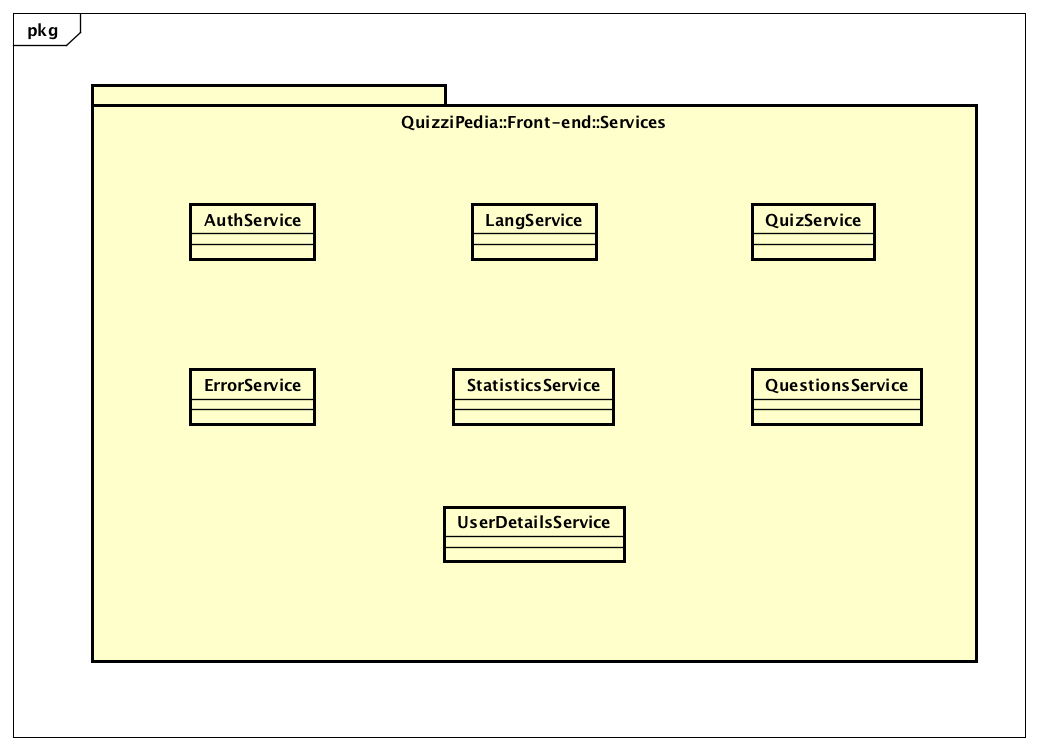
\includegraphics[scale=0.55]{UML/Package/QuizziPedia_Front-End_Services.png}
	\caption{QuizziPedia::Front-End::Services}
\end{figure} \FloatBarrier

\begin{itemize}
	\item \textbf{Descrizione}: package che contiene le classi individuate che permettono la comunicazione del lato front-end con il lato back-end;
	\item \textbf{Padre:} \texttt{Front-End};
	\item \textbf{Interazione con altri componenti:}
	\begin{itemize}
		\item \texttt{Models}: package che contiene le classi \textit{model\ped{G}} dell'applicazione;
		\item \texttt{Controllers}: package che contiene le classi \textit{controller\ped{G}} dell'applicazione.
	\end{itemize}
	\item \textbf{Classi contenute}:
	\begin{itemize}
		\item \texttt{AuthServices}: questa classe permette di gestire la registrazione e l'autenticazione di un utente;
		\item \texttt{LangService}: questa classe permette di gestire la lingua nella quale si è scelto di utilizzare l'applicazione;
		\item \texttt{QuestionsService}: questa classe permette di ottenere domande esistenti e salvare nuove domande;
		\item \texttt{QuizService}: questa classe permette di ottenere i dati di un quiz tramite delle parole chiave inserite dall'utente nella barra di ricerca. Permette inoltre di iscriversi ad un questionario e di scaricare l'intera lista di domande di un questionario a partire dal suo id univoco;
		\item \texttt{SearchService}: questa classe permette di gestire il recupero dei dati dal back-end a seguito di una ricerca effettuata da un utente;
		\item \texttt{StatisticsService}: questa classe permette di ottenere le statistiche dell'utente;
		\item \texttt{UserDetailsService}: questa classe permette di ottenere i dati personali degli utenti.
	\end{itemize} 
\end{itemize}
\newpage

\subsection{QuizziPedia::Front-End::Directives}

\label{QuizziPedia::Front-End::Directives}
\begin{figure} [ht]
	\centering
	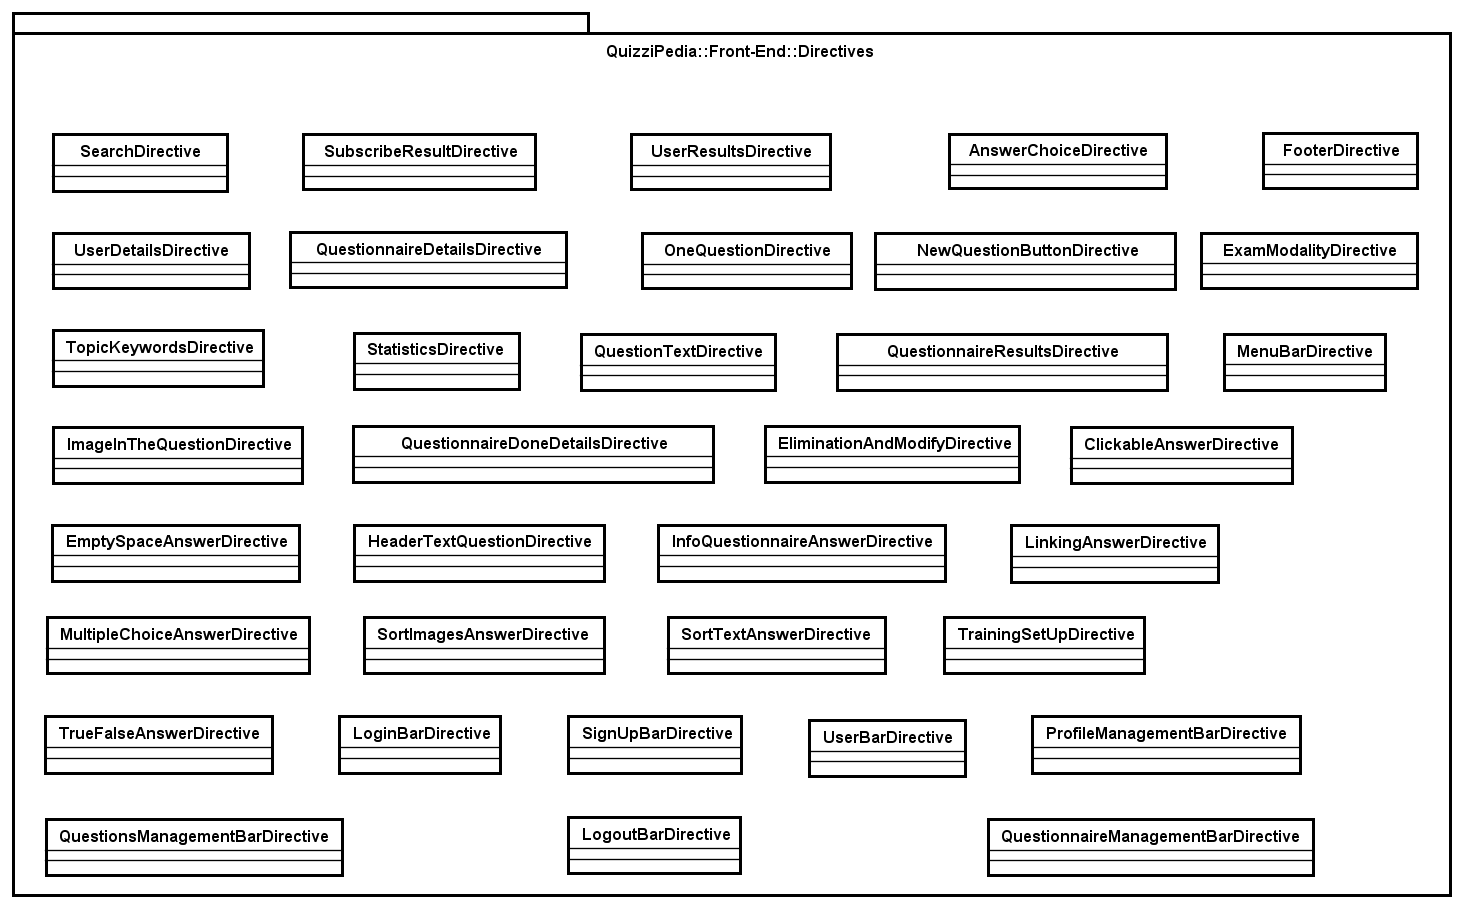
\includegraphics[scale=0.40]{UML/Package/QuizziPedia_Front-End_Directives.png}
	\caption{QuizziPedia::Front-End::Directives}
\end{figure}

\begin{itemize}
	\item \textbf{Descrizione}: package contenente le \textit{directives\ped{G}};
	\item \textbf{Padre}: \texttt{Front-End};
	\item \textbf{Interazione con altri componenti}:
	\begin{itemize}
		\item \texttt{Controllers}: package contenente i \textit{controllers\ped{G}} front-end dell'applicazione;
		\item \texttt{Views}: package contenente le \textit{views\ped{G}} front-end dell'applicazione.
	\end{itemize}
	\item \textbf{Classe contenute}:
	\begin{itemize}
		\item \texttt{EliminationAndModifyDirective}: componente grafico contenente i bottoni per eliminare o modificare un questionario;
		\item \texttt{ExamModalityDirective}: classe contenete i componenti grafici per attivare la modalità esame su un questionario e gestire le iscrizioni;
		\item \texttt{FooterDirective}: classe contenente i componenti grafici del footer dell'applicazione;
		\item \texttt{ImageInTheQuestionDirective}: classe contenente i componenti grafici per l'inserimento dell'immagine	nella creazione delle domande;
		\item \texttt{MenuBarDirective}: rappresenta il menù, presente in ogni pagina dell'applicazione, generato in base agli oggetti passati nello \$scope isolato. Fornisce un pulsante per ogni oggetto ricevuto come parametro, ogni pulsante viene rappresentato con un'icona e con un testo. Al click di un pulsante viene invocata la funzione ad esso associata;
		\item \texttt{OneQuestionDirective}: rappresenta il componente grafico che visualizza all'utente l'anteprima della domanda che ha creato. Eseguendo l'azione di click sul pulsante di modifica sarà possibile modificare tale domanda. All'interno di QuestionsManagementsView verranno stampati a video tanti componenti quanti presenti nello \$scope isolato ad esso associato;
		\item \texttt{NewQuestionButtonDirective}: rappresenta il componente grafico che permette all'utente di posizionarsi nella \textit{view\ped{G}} di creazione di una nuova domanda;
		\item \texttt{QuestionTextDirective}: rappresenta il componente grafico che permette all'utente di scrivere o modificare il testo di una domanda;
		\item \texttt{QuestionnaireDetailsDirective}: rappresenta il componente grafico che permette all'utente di visualizzare la lista di questionari che può compilare;
		\item \texttt{QuestionnaireDoneDetailsDirective}: rappresenta il componente grafico che permette all'utente di visualizzare la lista di questionari che ha già compilato e di conseguenza vederne le valutazioni;
		\item \texttt{QuestionnaireResultsDirective}: rappresenta il componente grafico che permette all'utente autenticato pro di vedere i risultati di chi ha compilato il questionario. Tale componente è contenuto nella lista dei questionari abilitati alla compilazione. É possibile accedere alla lista dei risultati azionando l'evento ad esso collegato;
		\item \texttt{QuestionnaireResultsDirective}: rappresenta il componente grafico che permette all'utente autenticato pro di vedere i risultati di chi ha compilato il questionario. Tale componente è contenuto nella lista dei questionari abilitati alla compilazione. É possibile accedere alla lista dei risultati azionando l'evento ad esso collegato;
		\item \texttt{SearchDirective}: classe che permette di effettuare la ricerca di utenti e questionari;
		\item \texttt{StatisticsDirective}: classe che permette di visualizzare le statistiche di un utente;
		\item \texttt{SubscribeResultDirective}: classe che permette di visualizzare e iscriversi ai questionari ricercati;
		\item \texttt{TopicKeywordsDirective}: classe che permette di gestire l'inserimento dell'argomento e delle	keywords al momento della creazione della domanda;
		\item \texttt{UserDetailsDirective}: classe che permette di visualizzare i dati personali di un utente;
		\item \texttt{UserResultsDirective}: classe che permette di visualizzare la lista degli utenti ricercati dopo aver utilizzato l'apposita funzione di ricerca;
		\item \texttt{ClickableAnswerDirective}: rappresenta il componente grafico che permette all'utente di visualizzare la domanda ad area cliccabile nell'immagine;
		\item \texttt{EmptySpaceAnswerDirective}: rappresenta il componente grafico che permette all'utente di visualizzare l'esercizio a riempimento di spazi vuoti;
		\item \texttt{HeaderTextQuestionDirective}: rappresenta componente grafico che presenta all'utente l'argomento e le parole chiave della domanda che ha a schermo;
		\item \texttt{InfoQuestionnaireDirective}: rappresenta il componente grafico che permette all'utente di visualizzare le informazioni principali del questionario che si sta per svolgere;
		\item \texttt{LinkingAnswerDirective}: rappresenta componente grafico che permette all'utente di visualizzare la domanda di collegamento;
		\item \texttt{MultipleChoiceAnswerDirective}: rappresenta componente grafico che permette all'utente di visualizzare la domanda a risposta multipla;
		\item \texttt{SortImagesAnswerDirective}: rappresenta il componente grafico che permette all'utente di visualizzare la domanda ad ordinamento di immagini;
		\item \texttt{SortTextAnswerDirective}: rappresenta il componente grafico che permette all'utente di visualizzare la domanda ad ordinamento di stringhe;
		\item \texttt{TrainingSetUpDirective}: rappresenta componente grafico che permette all'utente di selezionare l'argomento e le parole chiave per iniziare un allenamento con queste caratteristiche;
		\item \texttt{TrueFalseAnswerDirective}: rappresenta il componente grafico che permette all'utente di visualizzare la domanda vero e falso;
		\item \texttt{LoginBarDirective}: directive contenente il componente che permette di effettuare il redirect alla pagina di login;
		\item \texttt{SignUpBarDirective}: directive contenente il componente che permette di effettuare il redirect alla pagina di registrazione;
		\item \texttt{UserBarDirective}: directive contenente il componente che permette di effettuare il redirect alla pagina di visualizzazione profilo;
		\item \texttt{ProfileManagementBarDirective}: directive contenente il componente che permette di effettuare il redirect alla pagina di gestione del profilo;
		\item \texttt{QuestionsManagementBarDirective}: directive contenente il componente che permette di effettuare il redirect alla pagina di gestione delle domande;
		\item \texttt{LogoutBarDirective}: directive contenente il componente che permette di effettuare il logout dal sistema;
		\item \texttt{QuestionnaireManagementBarDirective}: directive contenente il componente che permette di effettuare il redirect alla pagina di gestione dei questionari.
	\end{itemize}
\end{itemize}
%\newpage

\subsection{QuizziPedia::Front-End::Models}

	\label{QuizziPedia::Front-End::Models}
	
	\begin{figure}[ht]
		\centering
		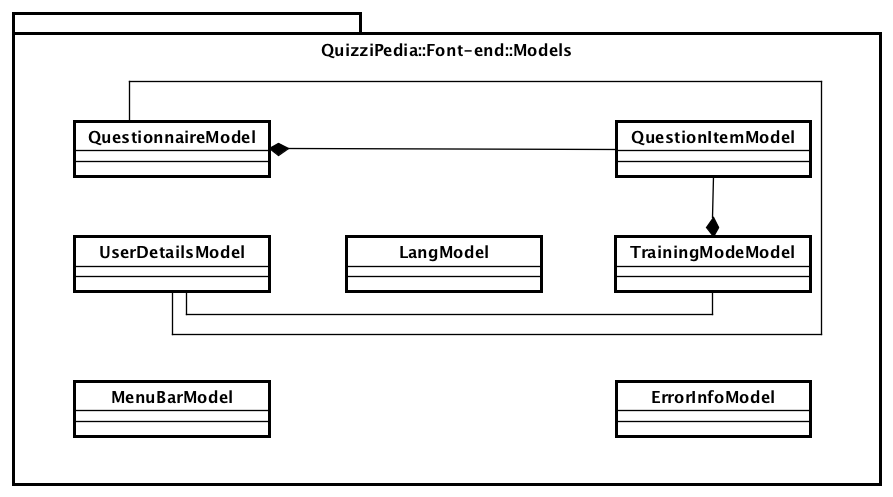
\includegraphics[scale=0.5,keepaspectratio]{UML/Package/QuizziPedia_Front-End_Models.png}
		\caption{QuizziPedia::Front-End::Models}
	\end{figure} \FloatBarrier

		\begin{itemize}
			\item \textbf{Descrizione}: \textit{package\ped{G}} contenente le classi che definiscono la business logic dell'applicazione;
			\item \textbf{Padre}: \texttt{Front-End};
			\item \textbf{Iterazioni con altri componenti}: 
				\begin{itemize}				
					\item \texttt{Controllers}: \textit{package\ped{G}} contenente i controllers front-end dell'applicazione;
					\item \texttt{Directives}: \textit{package\ped{G}} contenente le directives front-end dell'applicazione;
					\item \texttt{Models}: \textit{package\ped{G}} contenente le classi che definiscono la business logic dell'applicazione;
					\item \texttt{Services}: \textit{package\ped{G}} che contiene le classi individuate che permettono la comunicazione del lato front-end con il lato back-end attraverso l'architettura \textit{REST\ped{G}}.
				\end{itemize}
			\item \textbf{Classi contenute}:
			\begin{itemize}
				\item \texttt{UserDetailsModel}: rappresenta un utente. Contiene tutte le informazioni necessarie alla presentazione del contenuto di un utente sia nella visualizzazione che nella gestione di un profilo;
				\item \texttt{TrainingModeModel}: rappresenta un allenamento. Contiene tutte le informazioni necessarie alla presentazione del contenuto di un allenamento;
				\item \texttt{QuestionnaireModel}: rappresenta un questionario. Contiene tutte le informazioni necessarie alla presentazione del contenuto del questionario;
				\item \texttt{QuestionItemModel}: rappresenta una domanda. Contiene tutte le informazioni necessarie alla presentazione del contenuto della domanda;
				\item \texttt{MenuBarModel}: questa classe racchiude i dati necessari per la creazione dinamica della barra menù posizionata in modo fisso su ogni pagina;
				\item \texttt{LangModel}: rappresenta le informazioni per la giusta traduzione dell'applicazione;
				\item \texttt{ErrorInfoModel}: rappresenta le informazioni di un errore che si è verificato eseguendo una determinata operazione;
			\end{itemize}
		\end{itemize}

\newpage
\section{Specifica del Back-End}
\subsection{QuizziPedia::Back-End}
\subsubsection{Informazioni generali}
\label{QuizziPedia::Back-End}
\begin{figure}
	\centering
	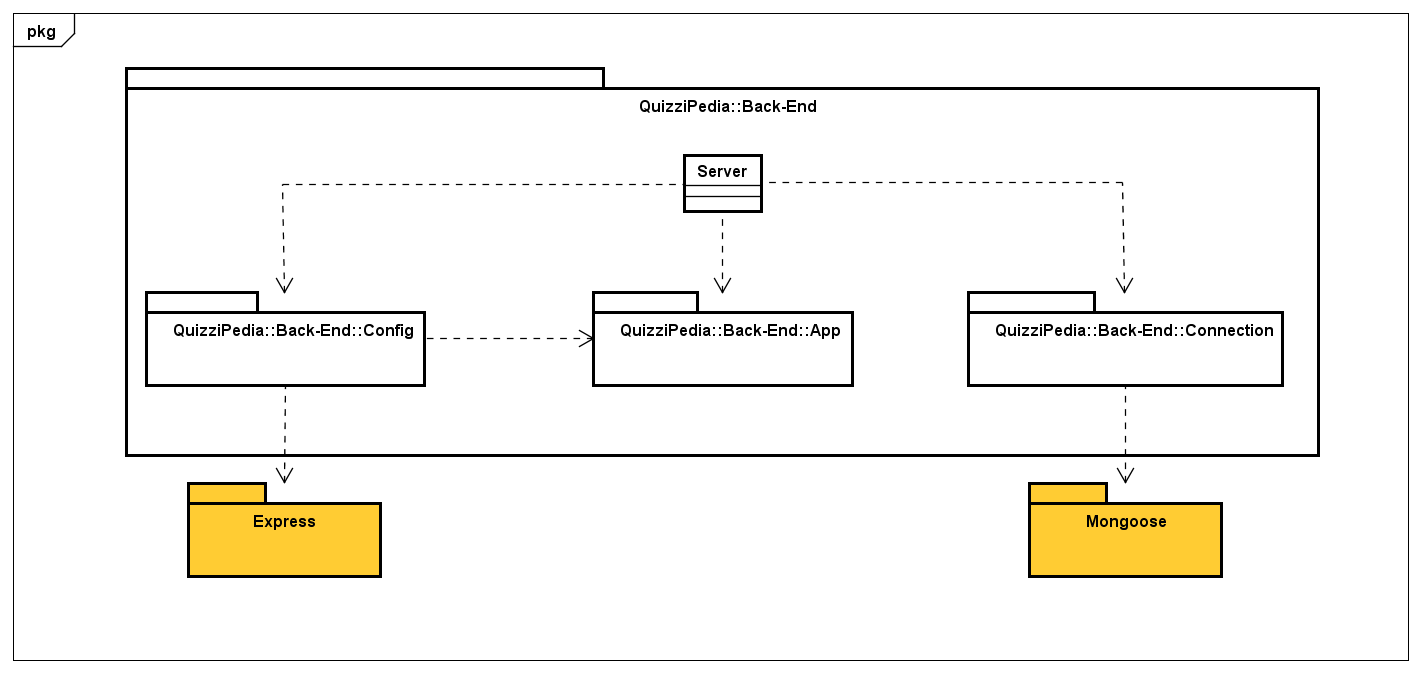
\includegraphics[scale=0.45]{UML/Package/QuizziPedia_Back-End.png}
	\caption{QuizziPedia::Back-End}
\end{figure}

	\begin{itemize}
		\item \textbf{Descrizione} \\ Package contenenti le componenti della parte back-end dell' applicazione.
		\item \textbf{Package contenuti}
		\begin{itemize}
			\item App \\
			Package\ped{G} contenente le componenti del server che implementano il \textit{pattern MVC\ped{G}}.
			\item Config \\
			Package\ped{G} contenente le componenti di configurazione del server\ped{G}.
		\end{itemize}
	\end{itemize}
\subsubsection{Classi}
	\paragraph{QuizziPedia::Back-End::Server}
	\begin{itemize}
		\item \textbf{Descrizione}
		\item \textbf{Utilizzo}
		\item \textbf{Relazioni con altre classi}
		\item \textbf{Attributi}
		\item \textbf{Metodi}
	\end{itemize}

\subsection{QuizziPedia::Back-End::Connection}
\subsubsection{Informazioni generali}
\subsubsection{Classi}

\subsection{QuizziPedia::Back-End::App}
\subsubsection{Informazioni generali}
\label{QuizziPedia::Back-End::App}
\begin{figure}
	\centering
	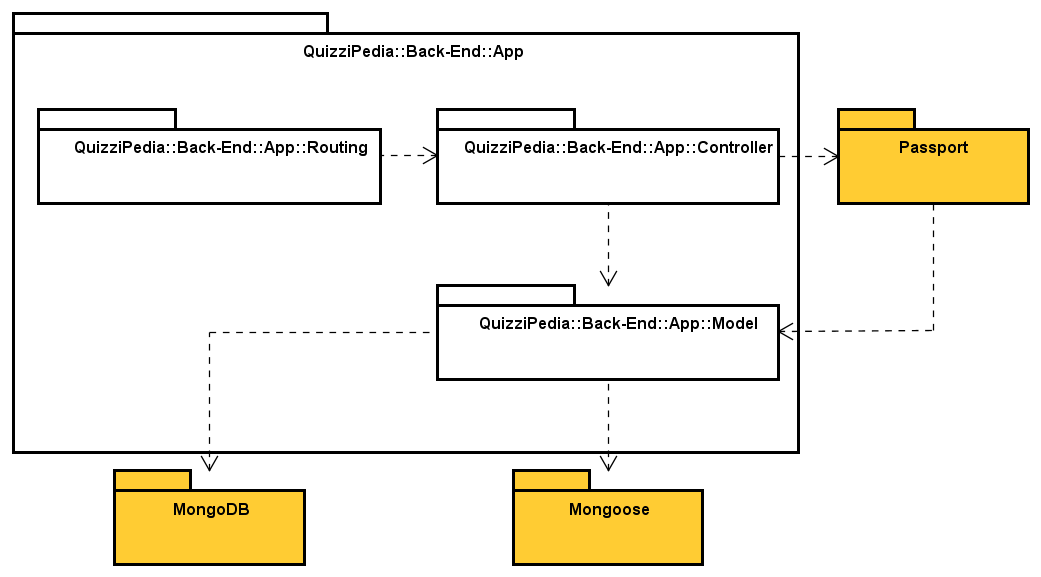
\includegraphics[scale=0.45]{UML/Package/QuizziPedia_Back-End_App.png}
	\caption{QuizziPedia::Back-End::App}
\end{figure}
	\begin{itemize}
		\item \textbf{Descrizione} \\
		Package contenente le componenti del server che implementano il \textit{pattern\ped{G} MVC\ped{G}};
		\item \textbf{Padre} \\ Back-End;
		\item \textbf{Interazioni con altri componenti}
			\begin{itemize}
				\item Congif \\
				Package contenente le componenti di configurazione del server;
			\end{itemize}
		\item \textbf{Package contenuti}
			\begin{itemize}
				\item Controllers \\
				Package che contiene i controllers di Express, definisce la logica dell'applicazione;
				\item Models \\
				Package che contiene le classi che definiscono il model dell'applicazione. Queste classi cono definite come classi schema di \textit{Mongoose\ped{G}}, il quale permette di utilizzare \textit{MongoDB\ped{G}} tramite degli oggetti;
				\item Routers \\
				Package contenente i routers della componente back-end dell'applicazione. Contiene i file di configurazione relativi al routing delle richieste del client, ossia i routers di Express.
			\end{itemize}
	\end{itemize}
	
\subsection{QuizziPedia::Back-End::App::Controllers}
\subsubsection{Informazioni generali}
	\begin{itemize}
		\item \textbf{Descrizione} \\
		\item \textbf{Padre} \\
		\item \textbf{Interazioni con altri componenti} \\
		\item \textbf{Package contenuti}
	\end{itemize}
\subsubsection{Classi}
\paragraph{QuizziPedia::Back-End::App::Controllers::NOMECLASSE}
	\begin{itemize}
		\item \textbf{Descrizione} \\
		\item \textbf{Utilizzo} \\
		\item \textbf{Relazioni con altre classi} \\
		\item \textbf{Metodi} \\
	\end{itemize}


\subsection{QuizziPedia::Back-End::App::Models}
\subsubsection{Informazioni generali}
\subsubsection{Classi}
\paragraph{QuizziPedia::Back-End::App::Models::NOMECLASSE}
\begin{itemize}
	\item \textbf{Descrizione} \\
	\item \textbf{Utilizzo} \\
	\item \textbf{Relazioni con altre classi} \\
	\item \textbf{Metodi} \\
\end{itemize}

\subsection{QuizziPedia::Back-End::App::Routers}
\subsubsection{Informazioni generali}
\subsubsection{classi}
\paragraph{QuizziPedia::Back-End::App::Routers::NOMECLASSE}
	\begin{itemize}
		\item \textbf{Descrizione} \\
		\item \textbf{Utilizzo} \\
		\item \textbf{Relazioni con altre classi} \\
		\item \textbf{Metodi} \\
<<<<<<< HEAD
	\end{itemize}
=======
	\end{itemize}
>>>>>>> origin/master

\appendix
\newpage
\section{Design patterns}

\subsection{Strutturali}
\subsubsection{Facade}
\textbf{Scopo}	Permette, attraverso un'interfaccia più semplice, l'accesso a sottosistemi che espongono interfacce complesse e molto diverse tra loro, nonché a blocchi di codice complessi. Questo rende una libreria più facile da capire, usare e testare, inoltre permette di diminuire le dipendenze tra sottosistemi senza nascondere le funzionalità di basso livello.
\\\\
\textbf{Motivazione}	L'utilizzo del pattern \textit{Facade\ped{G}} permette di nascondere la complessità del'operazione. Quando un sistema complesso viene strutturato in sottosistemi, le dipendenze rischiano di aumentare in modo consistente. Applicare il pattern \textit{Facede\ped{G}} aiuta a diminuire queste dipendenze. Il sottosistema possederà un'interfaccia semplificata che il \textit{client\ped{G}} utilizza anziché dover gestire numerosi oggetti. Utilizzare il pattern \textit{Facade\ped{G}} promuove un accoppiamento debole tra sottosistema ed i \textit{client\ped{G}}, che comporta una maggiore flessibilità nello sviluppo: è possibile modificare il sottosistema senza che i \textit{client\ped{G}} debbano adeguarsi a loro volta. \\
Ciononostante i \textit{client\ped{G}} possono comunque accedere alle funzionalità di basso livello ed utilizzare le classi del sottosistema.
\\\\
\textbf{Applicabilità}	Il pattern \textit{Facade\ped{G}} si usa nei seguenti casi:
	\begin{itemize}
		\item Si vuole fornire una singola interfaccia semplice per un sottosistema complesso;
		\item Si vuole promuovere il disaccoppiamento tra sottosistemi e \textit{client\ped{G}}, semplificando le dipendenze;
		\item Si vuole stratificare un sistema: è possibile definire una classe \textit{Facade\ped{G}} come punto d'ingresso per ogni livello di sottosistema. In questo modo, se vi sono dipendenze fra sottosistemi, essi possono comunicare fra loro attraverso la propria \textit{Facade\ped{G}}.
	\end{itemize}
\textbf{Utilizzo}

\subsection{Creazionali}
\subsubsection{Dependecy Injection}
\textbf{Scopo}	Semplificare lo sviluppo e rendere più testabile un software di grandi dimensioni. Il pattern \textit{Dependency Injection\ped{G}} separa il codice della componente dal codice che si occupa di risolvere le dipendenze con altre componenti.
\\\\
\textbf{Motivazione}	Lasciare al componente il compito di risolvere le proprie dipendenze, creando gli oggetti necessari al suo funzionamento, aumenta l'accoppiamento tra le componenti e rende più difficoltoso progettare i test di unità.
\\ Con questo pattern invece è possibile esprimere le dipendenze in modo dichiarativo e utilizzare un oggetto \textit{contenitore} per risolverle dinamicamente a \textit{runtime\ped{G}}. In questo modo è possibile scegliere anche quale componente iniettare in base allo stato del programma.
\\\\
\textbf{Applicabilità}	Questo pattern viene utilizzato dalla maggior parte dei \textit{framework\ped{G}} moderni. In particolare, \textit{AngularJS\ped{G}} offre il servizio
\\\\
\texttt{injector} che permette di invocare delle funzioni iniettando al loro interno degli oggetti.
\\\\
\textbf{Utilizzo}
\\\\
\textbf{Struttura}	I componenti coinvolti nel \textit{Dependency Injection} sono:
	\begin{itemize}
		\item Un \textit{client\ped{G}} che viene creato e riceve le dipendenze;
		\item Un \textit{contenitore} che si occupa di creare il \textit{client\ped{G}} e di iniettarvi le dipendenze;
		\item Un \textit{servizio} che deve essere iniettato al \textit{client\ped{G}}.
	\end{itemize}
Nello specifico di \textit{AngularJS\ped{G}} \texttt{Injector} funziona da \textit{contenitore} che si occupa di risolvere le dipendenze. I \textit{client\ped{G}} sono rappresentati dalle funzioni che costruiscono i componenti dell'applicazione, tipicamente \textit{controller\ped{G}} o \textit{service\ped{G}}. Il \textit{servizio} è un oggetto \textit{service} che può essere definito dall'utente oppure uno di quelli resi disponibili da \textit{AngularJS\ped{G}}.
\label{Struttura logica del pattern Dependency Injection}
\begin{figure}
	\centering
	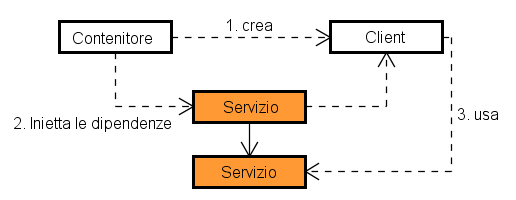
\includegraphics[scale=0.45]{UML/Package/strutturaPattern/DependencyInjection.png}
	\caption{Struttura logica del pattern Dependency Injection}
\end{figure}
\\\\
\textbf{Collaborazioni}
\\\\
\textbf{Svantaggi}	Eventuali errori legati alla risoluzione delle dipendenze o alla loro implementazione vengono rilevati solamente a \textit{runtime\ped{G}}.


\subsection{Comportamentali}
\subsubsection{Iterator}
\textbf{Scopo}	Il design pattern \textit{iterator\ped{G}} risolve diversi problemi connessi all'accesso e alla navigazione attraverso gli elementi di una struttura dati contenitrice, senza esporre i dettagli dell'implementazione e della struttura interna del contenitore
\\\\
\textbf{Motivazione}	Un'alternativa semplice e preferibile all'uso di indici (come accade ad esempio per gli array) consiste nell'aggiungere operazioni all'interfaccia del contenitore. Questa soluzione ha il grosso vantaggio che, se l'interfaccia è ben definita, consente di annullare la dipendenza da dettagli interni del contenitore, ma ciò presenta alcuni inconvenienti:
	\begin{itemize}
		\item \textit{Sovraccarico del'interfaccia del contenitore:} le operazioni aggiunte sovraccaricano l'interfaccia preesistente della classe contenitore;
		\item \textit{Mancanza di punti di accesso multipli:} le operazioni sono centralizzate nella classe contenitore. Questo non consente di effettuare contemporaneamente più visite indipendenti dagli elementi dello stesso contenitore;
		\item \textit{Supporto carente per metodi di navigazione specializzati:} quando i contenitori possiedono una struttura complessa, non di rado vi sono diversi e ugualmente utili modi di attraversarne l'insieme degli elementi contenuti. Un'interfaccia centralizzata si adatta male a questa situazione, perché richiede l'aggiunta di più operazioni specializzate, esacerbando il problema del sovraccarico.
	\end{itemize}
\textbf{Applicabilità}	Il design pattern \textit{iterator\ped{G}}, quindi, supera le soluzioni che si possono ottenere con la pura programmazione ad oggetti mediante codice più complesso.
\\
\textbf{Utilizzo}
\\\\
\textbf{Struttura}	Il pattern \textit{iterator\ped{G}} definisce due gerarchie di classi: una per i contenitori e una per gli iteratori\ped{G}. Le classi contenitore possono essere specializzate per tipo di elemento contenuto o per tipo di struttura in cui gli elementi sono organizzati. Le classi di iteratori\ped{G} sono specializzati per tipo di contenitore (iteratore\ped{G} concreto) e per tipo di navigazione attraverso la sequenza di elementi (iteratori\ped{G} specializzati).
\\
\label{Struttura logica del pattern Iterator}
\begin{figure}
	\centering
	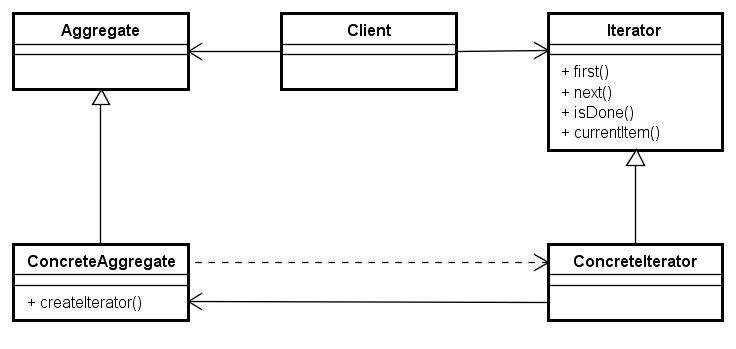
\includegraphics[scale=0.45]{UML/Package/strutturaPattern/Iterator.png}
	\caption{Struttura logica del pattern Iterator}
\end{figure}
\\
\textbf{Collaborazioni}	Il design pattern \textit{iterator\ped{G}} richiede la collaborazioni di alcuni elementi:
	\begin{itemize}
		\item \textbf{Iterator:} definisce un'interfaccia per attraversare l'insieme degli elementi di un contenitore e accedere ai singoli elementi;
		\item \textbf{ConcreteIterator:} implementa l'interfaccia \textit{iterator\ped{G}} tenendo traccia della posizione corrente nel contenitore e calcolando qual'è l'elemento successivo nella sequenza di attraversamento;
		\item \textbf{Aggregate:} definisce un'interfaccia per creare un oggetto \textit{iterator\ped{G}}.
		\item \textbf{ConcreteAggregate:} implementa l'interfaccia di creazione dell'\textit{iterator} e ritorna un'istanza appropriata di \texttt{ConcreteIterator}.
	\end{itemize}
\textbf{Svantaggi}	L'utilizzo del design pattern \textit{iterator\ped{G}} rende più complesso il codice e di conseguenza meno leggibile.


\subsubsection{Observer}
\textbf{Scopo}	Definisce una dipendenza “1..n” fra oggetti, riflettendo la modifica di un oggetto sui dipendenti.
\\\\
\textbf{Motivazione}	Il design pattern \textit{observer\ped{G}} verrà utilizzato per mantenere la consistenza fra oggetti. Il pattern definisce come implementare la relazione di dipendenza:
	\begin{itemize}
		\item \textit{Subject}: effettua le notifiche;
		\item \textit{Observer}: si aggiorna in risposta ad una notifica.
	\end{itemize}
\textbf{Applicabilità}	
\\\\
\textbf{Utilizzo}
\\\\
\textbf{Struttura}
\\\\
\textbf{Collaborazioni}
\\\\
\textbf{Svantaggi}
\subsubsection{Strategy}
\textbf{Scopo}
\textbf{Motivazione}
\textbf{Applicabilità}
\textbf{Utilizzo}
\textbf{Struttura}
\textbf{Collaborazioni}
\textbf{Svantaggi}

\subsection{Architetturali}
\subsubsection{MVC}
\textbf{Scopo}
\textbf{Motivazione}
\textbf{Applicabilità}
\textbf{Utilizzo}
\textbf{Struttura}
\textbf{Collaborazioni}
\textbf{Svantaggi}

\newpage
\section{Interfaccia REST}
Per utilizzare il Web come piattaforma di elaborazione, l'interfaccia per il \textit{Back-End\ped{G}} del progetto \progetto è realizzata in stile \textit{RESTful\ped{G}}.
L'interfaccia \textit{REST\ped{G}} propone una visione del Web incentrata sul concetto di risorsa, per questo motivo è stato preferito a \textit{SOAP\ped{G}} che espone un insieme di metodi richiamabili da remoto da parte di un \textit{client\ped{G}}. Inoltre \textit{SOAP\ped{G}} sfrutta il protocollo \textit{HTTP\ped{G}} come semplice protocollo di trasporto; REST\ped{G} lo usa come  protocollo di livello applicativo, per questo ne utilizza appieno le potenzialità.
I dati scambiati mediante l'interfaccia \textit{REST\ped{G}} sono rappresentati in formato \textit{JSON\ped{G}}, che si integra facilmente con le tecnologie ed il linguaggio utilizzati per sviluppare \progetto.
Se lo scambio di dati avviene correttamente il \textit{server\ped{G}} può fornire in risposta un messaggio di conferma:
\begin{lstlisting}[language=json,firstnumber=1]
{
"status" : "ok"
}
\end{lstlisting}
\subsection{Errori}
In caso di errori il \textit{server\ped{G}} risponde con un messaggio d'errore in formato \textit{JSON\ped{G}}, definito secondo lo schema:
\begin{lstlisting}[language=json,firstnumber=1]
{
"code" : [codice dell'errore],
"title" : [titolo dell'errore],
"message" : [descrizione testuale dell'errore]
}
\end{lstlisting}
\subsubsection{Errori generici}
Gli errori generici cono gestiti dalla classe \texttt{ErrorHandler} ad eccezione dell'errore \texttt{404} che viene gestito da \texttt{NotFoundHandler}. In questo modo si ottiene una gestione degli errori più flessibile e modulare, in quanto è possibile inserire in coda allo stack di chiamate di ogni ruote la classe \texttt{NotFoundHandler}, riducendo così la complessità della classe \texttt{ErrorHandler}.

\paragraph{Errori lato server}
Nel caso si verifichi un errore lato server, questo risponde con un codice \textit{HTTP\ped{G}} del tipo \texttt{5xx}. Di seguito vengono specificati gli errori che possono essere sollevati:
	\begin{itemize}
		\item \texttt{500 Errore sconosciuto}: il messaggio descrive un errore generico del server che avviene quando si verifica una condizione non gestibile e quindi non identificabile con un errore specifico.
	\end{itemize}
\paragraph{Errori nelle richieste da parte del client}
Nel caso si verifichi un errore riguardo le richieste ricevute dal client, il server risponde con un codice \textit{HTTP\ped{G}} del tipo \texttt{4xx}. Di seguito vengono specificati gli errori che possono essere sollevati:
	\begin{itemize}
		\item \texttt{400}: il server non può gestire la richiesta in seguito ad una generica richiesta errata. Il contenuto del messaggio d'errore varia in base alla tipologia di richiesta ricevuta;
		\item \texttt{401}: Accesso non autorizzato;
		\item \texttt{404}: Pagina non trovata.
	\end{itemize}
\paragraph{Errori specifici di \progetto}
Questi errori rappresentano situazioni specifiche del sistema \progetto, sono quindi stati definiti dei codici personalizzati per questa tipologia di errori basandosi sull'idea dei codici d'errore \textit{HTTP\ped{G}} standard. I codici dei messaggi d'errore sono stati assegnati secondo diverse categorie, in modo da poter individuare facilmente quale componente dell'applicazione ha causato l'errore. Ad ogni categoria è stato assegnato successivamente un intervallo di codici possibili, evitando di utilizzare gli intervalli \texttt{4xx} e \texttt{5xx} per non creare ambiguità con i codici d'errore standard descritti nella sezione precedente.
Le categorie di errori definite sono le seguenti:
\begin{itemize}
	\item \texttt{1xx}: errori di autenticazione, registrazione, modifica su utente e del middleware \texttt{userById};
		\begin{itemize}
			\item \texttt{101}: credenziali non valide;
			\item \texttt{102}: password assente;
			\item \texttt{103}: password troppo corta;
			\item \texttt{104}: password uguale all'attuale;
			\item \texttt{105}: password e conferma password non coincidono;
			\item \texttt{111}: campo obbligatorio vuoto;
			\item \texttt{112}: username non disponibile;
			\item \texttt{113}: username non valido;
			\item \texttt{114}: indirizzo mail non valido;
			\item \texttt{121}: formato immagine non valido;
			\item \texttt{122}: immagine di dimensione troppo grande;
			\item \texttt{123}: errore nel caricamento dell'immagine;
		\end{itemize}
	\item \texttt{2xx}: errori del middleware \texttt{questionById};
	\item \texttt{3xx}: errori del middleware \texttt{topicById};
	\item \texttt{6xx}: errori del middleware \texttt{quizById};
	\item \texttt{7xx}: errori del middleware \texttt{summaryById};
	\item \texttt{8xx}: errori del controller \texttt{QuestionController};
	\item \texttt{9xx}: errori del controller \texttt{TopicController};
	\item \texttt{10xx}: errori del controller \texttt{QuizController};
	\item \texttt{11xx}: errori del controller \texttt{SummaryController};
	\item \texttt{12xx}: errori degli oggetti \texttt{QuestionModel}:
	\item \texttt{13xx}: errori degli oggetti \texttt{TopicModel};
	\item \texttt{14xx}: errori degli oggetti \texttt{QuizModel};
	\item \texttt{15xx}: errori degli oggetti \texttt{SummaryModel};
\end{itemize}
Gli errori specifici di \progetto vengono gestiti dalla classe \texttt{QuizziPediaError} e sono di seguito elencati sotto forma di:
\begin{center}
	\texttt{Codice Titolo}: messaggio d'errore
\end{center}
\begin{itemize}
	\item \texttt{100 Utente non trovato:} l'identificativo utente fornito non è un identificativo valido;
	\item \texttt{101 Credenziali non valide:} è necessario fornire un username ed una password valide;
	\item \texttt{102 Password assente:} è necessario inserire una password;
	\item \texttt{103 Password troppo corta:} è necessario inserire una password di almeno 6 caratteri;
	\item \texttt{104 Password uguale all'attuale:} è necessario inserire una password diversa della precedente;
	\item \texttt{105 Le password non coincidono:} è necessario che 'password' e 'conferma password' siano identiche;
	\item \texttt{111 Campo obbligatorio vuoto:} è necessario riempire tutti i campi obbligatori;
	\item \texttt{112 Username non disponibile:} l 'username è già stato utilizzato, prego inserire un nuovo username;
	\item \texttt{113 Username non valido:} l'username non è valido;
	\item \texttt{114 Indirizzo mail non valido: } è necessario fornire un indirizzo e-mail valido;
	\item \texttt{121 Formato immagine non valido: } Il formato dell'immagine non è valido;
	\item \texttt{122 Immagine di dimensione troppo grande: } La dimensione massima per l'immagine è di 20MB;
	\item \texttt{123 Caricamento immagine fallito}: errore sconosciuto nel caricamento dell'immagine;
	\item \texttt{200 Domanda non valida:} l'identificativo della domanda fornita non è un identificativo valido;
	\item \texttt{300 Argomento non valido:} l'identificativo dell'argomento fornito non è un identificativo valido;
	\item \texttt{600 Questionario non valido:}  l'identificativo del questionario fornito non è un identificativo valido;
	\item \texttt{700 Sommario non valido:} l'identificativo del questionario fornito non è un identificativo valido;
	\item \texttt{800 Dati non validi:} i dati relativi al contenuto della domanda non sono  validi o sono formattati in modo errato;
	\item \texttt{900 Dati non validi:} i dati relativi al contenuto dell'argomento non sono validi;
	\item \texttt{1000 Dati non validi:} i dati relativi al contenuto del questionario non validi;
	\item \texttt{1100 Dati non validi:} i dati relativi al contenuto del  sommario non validi o sono formattati in modo errato;
	\item \texttt{1200 Dati non validi:} i dati per la modifica di una domanda non sono definiti;
	\item \texttt{1300 Dati non validi:} i dati per la gestione dell' argomento non sono definiti;
	\item \texttt{1400 dati non validi:} i dati per la gestione del questionario non sono definiti;
	\item \texttt{1500 Dati non validi:} i dati per la gestione del sommario non sono validi;
\end{itemize}

\subsection{Risorse REST}
In seguito vengono riportate le risorse \textit{REST\ped{G}} fornite, associate al tipo di metodo \textit{HTTP\ped{G}} che è possibile richiedere su di esse e ai permessi necessari per effettuare la richiesta. In particolare, i permessi sono:
\begin{itemize}
	\item \textbf{Utente}: la risorsa può essere acceduta da qualsiasi tipo di utente;
	\item \textbf{Utente autenticato}: la risorsa può essere acceduta solo dagli utenti che hanno effettuato il login;
	\item \textbf{Utente autenticato pro}: la risorsa può essere acceduta solo dagli utenti pro.
\end{itemize}
Inoltre per ogni risorsa sono stati specificati i formati per lo scambio dei dati in JSON\ped{G}:
\begin{itemize}
	\item \textbf{Request}: rappresenta l'oggetto \textit{JSON\ped{G}} che dovrà essere passato alla risorsa \textit{REST\ped{G}};
	\item \textbf{Response}: rappresenta l'oggetto \textit{JSON\ped{G}} che fornirà in risposta la risorsa \textit{REST\ped{G}};
		\item \texttt{/:lang}
		\begin{itemize}
			\item \textbf{Method}: GET
			\item \textbf{Livello di Accesso}: Utente;
			\item \textbf{Descrizione}: restituisce le keywords inerenti alla lingua impostata
			\item \textbf{Response}: la risposta deve avere i seguenti campi:
\begin{lstlisting}[language=json,firstnumber=1]
{
"keywords": [Array contenente le keywords inerenti alla lingua impostata ]
}
\end{lstlisting}
		\end{itemize}
	
	
	\item \texttt{/:lang/signup}
		\begin{itemize}
			\item \textbf{Method}: POST
			\item \textbf{Livello di Accesso}: Utente;
			\item \textbf{Descrizione}: crea un nuovo account. Un username univoco inserito dall'utente lo identifica, pertanto non ci saranno più utenti con lo stesso username. Restituisce un messaggio di conferma se viene effettuato correttamente, altrimenti un errore.
			\item \textbf{Request}: lo scambio dei dati dell'utente avviene attraverso una form che deve avere i seguenti campi:
\begin{lstlisting}[language=json,firstnumber=1]
{
"username" : [username univoco scelto dall'utente]
"password" : [la password associata all'account che si vuole registrare]
"e-mail" : [l'indirizzo e-mail con cui si effettua la registrazione]
"name" : [nome dell'utente da registrare]
"surname" : [cognome dell'utente da registrare]
}
\end{lstlisting}
		\end{itemize}
		\item \texttt{/signin}
		\begin{itemize}
			\item \textbf{Method}: POST;
			\item \textbf{Livello di Accesso}: utente/utente pro;
			\item \textbf{descrizione}: effettua l'accesso all'account. Restituisce un messaggio di conferma se viene effettuato correttamente, altrimenti un errore.
			\item \textbf{Request}: lo scambio dei dati dell'utente avviene attraverso una form che deve avere i seguenti campi:
\begin{lstlisting}[language=json,firstnumber=1]
{
"username" : [username che corrisponde all'username inserita durante la registrazione]
"password" : [la password associata all'username dell'account dell'utente]
}
\end{lstlisting}
			\item \textbf{Response}: la risposta deve contenere i seguenti campi:
\begin{lstlisting}[language=json,firstnumber=1]
{
"_userId" : [identificativo dell'utente]
"username" : [username che corrisponde all'username inserita durante la registrazione]
}
\end{lstlisting}
		\end{itemize}
		\item \texttt{/signout}
		\begin{itemize}
			\item \textbf{Method}: GET;
			\item \textbf{Livello di Accesso}: Utente autenticato/autenticato pro;
			\item \textbf{Descrizione}: effettua il logout. restituisce un messaggio di conferma se viene effettuato correttamente, altrimenti un errore;
		\end{itemize}
		\item \texttt{/:lang/recovery}
		\begin{itemize}
			\item \textbf{Method}: POST;
			\item \textbf{Livello di Accesso}: Utente;
			\item \textbf{Descrizione}: invia una nuova password sulla mail dell'utente generata in automatico, restituisce un messaggio di conferma se viene effettuato correttamente, altrimenti un errore;
			\item \textbf{Request}: la richiesta di recupero della password deve avere i seguenti campi:
\begin{lstlisting}[language=json,firstnumber=1]
{
"e-mail" : [la password associata all'username dell'account dell'utente]
}
\end{lstlisting}
		\end{itemize}
		\item \texttt{/:lang/user/:userId/search/:keyword/users}
	 \begin{itemize}
	 	\item \textbf{Method}: GET;
	 	\item \textbf{Livello di Accesso:} Utente autenticato/autenticato pro;
	 	\item \textbf{Descrizione}: effettua una ricerca di utenti da parte di un utente;
	 	\item \textbf{Request}: la richiesta deve avere i seguenti campi:
\begin{lstlisting}[language=json,firstnumber=1]
{
"keyword" : [stringa da ricercare]
}
\end{lstlisting} 
		\item \textbf{Response:} la risposta deve avere un campo \texttt{array} contenente i risultati degli utenti trovati:
\begin{lstlisting}[language=json,firstnumber=1]
{
"userResult" : [
"_userID" : [identificativi dell'utente trovato]
"name" : [nome dell'utente trovato]
"surname" : [cognome dell'utente trovato]
]
}
\end{lstlisting}
	 \end{itemize}

\item \texttt{/:lang/user/:userId/search/:keyword/quizzes}
	 \begin{itemize}
	 	\item \textbf{Method}: GET;
	 	\item \textbf{Livello di Accesso:} Utente autenticato/autenticato pro;
	 	\item \textbf{Descrizione}: effettua una ricerca di questionari da parte di un utente;
	 	\item \textbf{Request}: la richiesta deve avere i seguenti campi:
\begin{lstlisting}[language=json,firstnumber=1]
{
"keyword" : [stringa da ricercare]
}
\end{lstlisting} 
		\item \textbf{Response:} la risposta deve avere un campo \texttt{array} contenente i risultati dei questionari trovati:
\begin{lstlisting}[language=json,firstnumber=1]
{
"quizResult : [
"_quizID" : [identificativo del questionario]
"title" : [titolo del questionario]
"author" : [username dell'autore del questionario]
]
}
\end{lstlisting}
	 \end{itemize}	 
	 
	\item \texttt{/:lang/user/:userId/search/users/:userId}
	 \begin{itemize}
	 	\item \textbf{Method}: GET;
	 	\item \textbf{Livello di Accesso:} Utente autenticato/autenticato pro;
	 	\item \textbf{Descrizione}: restituisce le informazioni dell'utente precedentemente trovato tramite una ricerca;
	 	\item \textbf{Response:} 
\begin{lstlisting}[language=json,firstnumber=1]
{
"username" : [username utente da visualizzare]
"name" : [nome utente da visualizzare]
"surname" : [cognome utente da visualizzare]
"email" : [email utente da visualizzare]
"userImg": [rappresenta l'immagine dell'utente da visualizzare]
"levelUser" : [livello utente da visualizzare]
"statistics":[array di JSON, contenente le statische dell'utente di ogni argomento]
}
\end{lstlisting}
	 \end{itemize}
	 
	 
	\item \texttt{/:lang/user/:userId/search/quizzes/:quizId}
	\begin{itemize}
		\item \textbf{Method}: GET;
		\item \textbf{Livello di Accesso:} Utente autenticato/autenticato pro;
		\item \textbf{Descrizione}: restituisce le informazioni del questionario precedentemente trovato tramite una ricerca;
		\item \textbf{Response:} 
\begin{lstlisting}[language=json,firstnumber=1]
{
"title" : [identifica il titolo del questionario]
"author" : [identifica l'autore del questionario]
"questions" : [identifica l'Array di JSON con le domande relative al questionario]
}
\end{lstlisting}
	\end{itemize}
	\item \texttt{/profile/:userId}
	\begin{itemize}
		\item \textbf{Method}: DELETE;
		\item \textbf{Livello di Accesso}: utente autenticato/autenticato pro;
		\item \textbf{Descrizione}: elimina l'utente autenticato con id pari a :userId. 		Restituisce un messaggio di conferma se viene effettuato correttamente, altrimenti un errore;
		\item \textbf{Response}:la risposta deve contenere i seguenti campi:
\begin{lstlisting}[language=json,firstnumber=1]
{
   	"name" : [identifica il nome dell'utente]
    	"surname" : [identifica il nome dell'utente]
}
\end{lstlisting}
	\end{itemize}	
	
	\item \texttt{/profile/info/:userId}
		\begin{itemize}
			\item \textbf{Method}: GET;
			\item \textbf{Livello di Accesso}: utente autenticato/autenticato pro;
			\item \textbf{Descrizione}: restituisce le informazioni riguardante l'utente autenticato con id pari a :userId. Restituisce un messaggio di conferma se viene
effettuato correttamente, altrimenti un errore;
			\item \textbf{Response}: la risposta deve contenere i seguenti campi:
\begin{lstlisting}[language=json,firstnumber=1]
{
	"username" : [username utente da visualizzare]
	"name" : [nome utente da visualizzare]
	"surname" : [cognome utente da visualizzare]
	"email" : [email utente da visualizzare]
	"userImg": [rappresenta l'immagine dell'utente da visualizzare]
	"levelUser" : [livello utente da visualizzare]
}
\end{lstlisting}
		\end{itemize}
		
	\item \texttt{/profile/info/:userId}
		\begin{itemize}
			\item \textbf{Method}: PUT;
			\item \textbf{Livello di Accesso}: utente autenticato/autenticato pro;
			\item \textbf{Descrizione}: modifica le informazioni riguardante l'utente autenticato con id pari a :userId. Restituisce un messaggio di conferma se viene
effettuato correttamente, altrimenti un errore;
			\item \textbf{Request}: la richiesta deve contenere i seguenti campi:
\begin{lstlisting}[language=json,firstnumber=1]
{
	"name" : [nome utente]
	"surname" : [cognome utente]
	"email" : [email utente]
	"userImg": [immagine profilo utente]
	"levelUser" : [livello utente]
}
\end{lstlisting}
		\end{itemize}	
		
	\item \texttt{/profile/info/privacy/:userId}
		\begin{itemize}
			\item \textbf{Method}: PUT;
			\item \textbf{Livello di Accesso}: utente autenticato/autenticato pro;
			\item \textbf{Descrizione}: modifica la password di accesso al sistema riguardante l'utente autenticato con id pari a :userId. Restituisce un messaggio di conferma se viene effettuato correttamente, altrimenti un errore;
			\item \textbf{Request}: la richiesta deve contenere i seguenti campi:	
\begin{lstlisting}[language=json,firstnumber=1]
{
    "password" : [identifica la nuova password inserita dallutente]
}	

\end{lstlisting}
		\end{itemize}
		
	\item \texttt{/profile/statistics/:userId}
		\begin{itemize}
			\item \textbf{Method}: GET;
			\item \textbf{Livello di Accesso}: utente autenticato/autenticato pro;
			\item \textbf{Descrizione}: restituisce le statistiche riguardanti l'utente autenticato con id pari a :userId. 
			\item \textbf{Response}: la risposta deve contenere i seguenti campi:	
\begin{lstlisting}[language=json,firstnumber=1]
{
    "name": [identifica il nome dell'utente]
    "surname": [identifica il nome dell'utente]
    "userImg": [rappresenta l'immagine dell'utente]
	"statistics":[array di JSON, contenente le statische dell'utente di ogni argomento]
	"summaries":[array di JSON contenente la cronologia dei questionari svolti dall'utente]   
}	

\end{lstlisting}
		\end{itemize}
	
	\item \texttt{/:lang/user/:userId/question}
	\begin{itemize}
		\item \textbf{Method}: GET;
		\item \textbf{Livello di Accesso}: Utente autenticato/autenticato pro;
		\item \textbf{Descrizione}: Restituisce le domande create dall'utente;
		\item \textbf{Response}: la risposta deve avere i seguenti campi:
\begin{lstlisting}[language=json,firstnumber=1]
{
"listQuestion" : [ 
"type" : [identifica tipologia domanda]
"language" : [identifica la lingua della domanda]
"questionText" : [identifica il testo della domanda]
"image" : [identifica l'immagine relativa al testo della domanda]
"option1" : [identifica l'array di opzioni di risposte]
"option2" : [identifica l'array di opzioni di risposte]
"totalAnswer" : [identifica il numero totale di risposte date alla domanda]
"correctAnswer" : [identifica il numero di risposte corrette date alla domanda]
]
}
\end{lstlisting}
	\end{itemize}	
	
	
	\item \texttt{/:lang/user/question}
		\begin{itemize}
			\item \textbf{Method}: POST;
			\item \textbf{Livello di Accesso}: Utente autenticato/autenticato pro;
			\item \textbf{Descrizione}: Aggiunge una domanda nel sistema, restituisce un messaggio di conferma o di errore;
			\item \textbf{Request}: la richiesta deve contenere i seguenti campi:
\begin{lstlisting}[language=json,firstnumber=1]
{
"listQuestion" : [ 
"type" : [identifica tipologia domanda]
"language" : [identifica la lingua della domanda]
"questionText" : [identifica il testo della domanda]
"image" : [identifica l'immagine relativa al testo della domanda]
"option1" : [identifica l'array di opzioni di risposte]
"option2" : [identifica l'array di opzioni di risposte]
]
}
\end{lstlisting}
		\end{itemize}
	\item \texttt{/:lang/user/:userId/quiz}
	\begin{itemize}
		\item \textbf{Method}: GET;
		\item \textbf{Livello di Accesso}: Utente autenticato pro;
		\item \textbf{Descrizione}: Restituisce i questionari creati dall'utente pro;
		\item \textbf{Response}: la risposta deve avere i seguenti campi:
\begin{lstlisting}[language=json,firstnumber=1]
{
"listQuiz" : [ 
"title" : [identifica il titolo del questionario]
"questions" : [Arrai di JSON contenente le domande relative al questionario]
]
}
\end{lstlisting}
	\end{itemize}	
	
	
	\item \texttt{/:lang/user/:userId/quiz}
		\begin{itemize}
			\item \textbf{Method}: POST;
			\item \textbf{Livello di Accesso}: Utente autenticato pro;
			\item \textbf{Descrizione}: Aggiunge un questionario nel sistema, restituisce un messaggio di conferma o di errore;
			\item \textbf{Request}: la richiesta deve contenere i seguenti campi:
\begin{lstlisting}[language=json,firstnumber=1]
{
"title" : [titolo del questionario]
"questions" : [Array di JSON contenente gli identificativi delle domande che compongono il questionario]
}
\end{lstlisting}
		\end{itemize}
		
		
	\item \texttt{/:lang/user/quiz/:quizId/addUser}
	\begin{itemize}
		\item \textbf{Method}: POST;
		\item \textbf{Livello di Accesso}: Utente autenticato pro;
		\item \textbf{Descrizione}: Iscrive un utente ad un questionario, restituisce un messaggio di conferma o di errore;
		\item \textbf{Request}: la richiesta deve contenere i seguenti campi:
\begin{lstlisting}[language=json,firstnumber=1]
{
"_userId" : [identificativo dell'utente da iscrivere al questionario]
}
\end{lstlisting}
	\end{itemize}
	
	\item \texttt{/:lang/user/quiz/:quizId/activeUser}
	\begin{itemize}
		\item \textbf{Method}: POST;
		\item \textbf{Livello di Accesso}: Utente autenticato/autenticato pro;
		\item \textbf{Descrizione}: Aggiunge un utente iscritto al questionario nella lista degli utenti che lo hanno eseguito;
		\item \textbf{Request}: la richiesta deve contenere i seguenti campi:
\begin{lstlisting}[language=json,firstnumber=1]
{
"_userId" : [identificativo dell'utente da iscrivere al questionario]
}
\end{lstlisting}
	\end{itemize}
	
	\item \texttt{/:lang/user/:userId/quiz/:quizId}
	\begin{itemize}
		\item \textbf{Method}: PUT;
		\item \textbf{Livello di Accesso}: Utente autenticato pro;
		\item \textbf{Descrizione}: Modifica in questionario creato in precedenza, restituisce un messaggio di conferma o di errore;
		\item \textbf{Request}: la richiesta deve contenere i seguenti campi:
\begin{lstlisting}[language=json,firstnumber=1]
{
"title" : [titolo del questionario]
"questions" : [Array di JSON contenente gli identificativi delle domande che compongono il questionario]
}
\end{lstlisting}
	\end{itemize}
	
	\item \texttt{/:lang/user/quiz/:quizId/test}
	\begin{itemize}
		\item \textbf{Method}: POST;
		\item \textbf{Livello di Accesso}: Utente autenticato/autenticato pro;
		\item \textbf{Descrizione}: Restituisce il quiz selezionato dall'utente per effettuare l'esercitazione
		\item \textbf{Response}: la richiesta deve contenere i seguenti campi:
\begin{lstlisting}[language=json,firstnumber=1]
{
"title" : [titolo del questionario]
"author" : [identifica l'autore del questionario]
"questions" : [Array di JSON contenente le domande che compongono il questionario]
}
\end{lstlisting}
	\end{itemize}
	
	
	\item \texttt{/:lang/user/quiz/:quizId/summary}
	\begin{itemize}
		\item \textbf{Method}: POST;
		\item \textbf{Livello di Accesso}: Utente autenticato/autenticato pro;
		\item \textbf{Descrizione}: Crea il riepilogo del questionario svolto;
		\item \textbf{Request}: la richiesta deve contenere i seguenti campi:
\begin{lstlisting}[language=json,firstnumber=1]
{
"_quizId" : [identificativo del questionario svolto]
"_userId" : [identificativo dell'utente che ha svolto il questionario]
"givenAnswers" : [Array di JSON contenente le domande del quiz associate alle risposte date dall'utente]
}
\end{lstlisting}
		\item \textbf{Response}: la risposta deve contenere i seguenti campi:
\begin{lstlisting}[language=json,firstnumber=1]
{
"mark" : [valutazione del questionario]
"answers" : [Array di JSON contenente le domande del quiz associate alle risposte date dall'utente e le risposte corrette]
}
\end{lstlisting}
	\end{itemize}
		\item \texttt{/:lang/training}
		\begin{itemize}
			\item \textbf{Method}: POST;
			\item \textbf{Livello di Accesso}: Utente;
			\item \textbf{Descrizione}: restituisce una domanda in base al livello di abilità raggiunto dall'utente;
			\item \textbf{Request}: la richiesta deve contenere i seguenti campi:
\begin{lstlisting}[language=json,firstnumber=1]
{
"topicTraining" : [indica l'argomento scelto per iniziare l'allenamento]
"numberQuestions" : [indica il numero di domande che componono l'allenamento]
"keyword" : [indica un array di parole chiavi per filtrare le domande]
"levelUser" : [indica il livello di abilita' sull'argomento scelto dell'utente]
}
\end{lstlisting}
			\item \textbf{Response}: la risposta deve contenere i seguenti campi:
\begin{lstlisting}[language=json,firstnumber=1]
{
"_questionId" : [identificativo della domanda]
"type" : [indica la tipologia della domanda]
"questionText" : [indica il testo della domanda]
"option1" : [indica un array di opzioni di risposta]
"option2" : [indica un array di opzioni di risposta] 
}
\end{lstlisting}
		\end{itemize}
		
		
	\item \texttt{/:lang/user/training}
		\begin{itemize}
			\item \textbf{Method}: POST;
			\item \textbf{Livello di Accesso}: Utente autenticato/autenticato pro;
			\item \textbf{Descrizione}: restituisce una domanda, aggiorna le statistiche della domanda e dell'utente;
			\item \textbf{Request}: la richiesta deve contenere i seguenti campi:
\begin{lstlisting}[language=json,firstnumber=1]
{
"topicTraining" : [indica l'argomento scelto per iniziare l'allenamento]
"numberQuestions" : [indica il numero di domande che componono l'allenamento]
"keyword" : [indica un array di parole chiavi per filtrare le domande]
"levelUser" : [indica il livello di abilita' sull'argomento scelto dell'utente]
}
\end{lstlisting}
		\item \textbf{Response}: la risposta deve contenere i seguenti campi:
\begin{lstlisting}[language=json,firstnumber=1]
{
"_questionId" : [identificativo della domanda]
"type" : [indica la tipologia della domanda]
"questionText" : [indica il testo della domanda]
"option1" : [indica un array di opzioni di risposta]
"option2" : [indica un array di opzioni di risposta] 
}
\end{lstlisting}
	\end{itemize}
\end{itemize}

\end{document}